\chapter{Diskretisierung}

\ac{pdgn} $n$-ter Ordnung für skalares $u(x)$ sind von der Form
\begin{equation}
  F(x, t, u(x), Du(x), \dots, D^nu(x))=0, \qquad x\in\Omega\subset\mathbb{R}^d \; .
\end{equation}
Sie unterliegen Randbedingungen (für die Zeitvariable auch Anfangsbedingung genannt), die je nach Problemstellung auf Teilen des Randes formuliert sind. Beispielsweise ist die Auslenkung einer eingespannten Membran am Ortsrand fest, während in der Zeit lediglich für $t_0$ ein Randwert vorliegt (am linksseitigen Rand der Zeitdomäne).

Die \ac{lvn} \eqref{eq:lvn} ist eine lineare \ac{pdg} zweiter Ordnung in $d=2$ Dimensionen. Sie ist weder elliptisch, noch parabolisch, noch hyperbolisch\footnote{Dies ist ersichtlich anhand der Eigenwerte der Koeffizientenmatrix zweiter Ableitungen $T=\text{diag}(0,1,-1)$ für Gleichung \eqref{eq:lvn_first}. Bei elliptischen Problemen haben alle Koeffizienten gleiches Vorzeichen und sind ungleich Null. Bei hyperbolischen Problemen hat genau ein Eigenwert ein anderes Vorzeichen und alle Koeffizienten sind ungleich Null. Parabolische Probleme schließlich sind gekennzeichnet durch genau einen Null-Eigenwert und ansonsten gleiches Vorzeichen.}.
Ferner bildet $u\in C^2(\Omega)$ in den Raum der komplexen Zahlen ab. Damit unterscheidet sich das Problem bereits grundlegend von den zumeist in der Literatur vorkommenden Problemstellungen. Die stationäre \ac{lvn} hingegen ist hyperbolisch. In diesem Kapitel soll ein Verfahren entwickelt werden, welches bislang noch nicht zur Anwendung gekommen ist im Kontext der \ac{lvn}: das \emph{\ac{dg}}-Verfahren\index{Discontinuous-Galerkin Verfahren}. Die Ausführungen orientieren sich an dem praxisnahen Buch von Hesthaven und Warburton \cite{buch}.

Zunächst wird ein Überblick über verschiedene, gängige numerische Verfahren gegeben. Vor- und Nachteile werden skizziert, wenngleich die Numerik partieller Differentialgleichungen ein großes Forschungsgebiet ist und somit die verschiedenen angedeuteten Probleme sich möglicherweise nur in einer oberflächlichen Betrachtung als solche äußern.

\section{Übersicht}\label{sec:Übersicht}
Bei der Diskretisierung einer \ac{pdg} sind zwei grundlegende Fragestellungen zu berücksichtigen:
\begin{enumerate}
  \item Auf welche Weise wird die Lösung $u(x,t)$ durch eine diskrete Lösung $u_h(x,t)$ genähert?
  \item Wie ist die Verbindung zwischen diskretisierter Lösung und zugrundeliegender \ac{pdg}?
\end{enumerate}
Als Folge einer unterschiedliche Beantwortung dieser Fragen wurden zahlreiche Verfahren entwickelt, die jeweils spezifische Vor- und Nachteile aufweisen. Im Folgenden werden in knapper Form drei Verfahren vorgestellt und  gegeneinander verglichen. In dieser Reihenfolge nimmt die Komplexität zu, denn die Schwächen des einen Verfahrens führen jeweils zu der nächst allgemeineren Formulierung.

\subsection{Finite Differenzen}\index{Finite Differenzen}\label{sec:FD}
Die partiellen Ableitungen werden bei diesem Verfahren durch eine endliche (finite) Anzahl von Differenzen genähert. Zur Formulierung der n-ten Ableitung einer Funktion $f(x)$ im Punkt $x_0$ wird die zugehörige Taylorreihe bis zur n-ten Ordnung verwendet. Der Punkt $x_0$ entstammt einem Gitter, welches das Gebiet $\Omega$ diskretisiert. Dieser Ansatz setzt inhärent voraus, dass eine Funktion sich hinreichend genau durch ein lokales Polynom niedriger Ordnung nähern lässt. Damit ist zeitgleich Frage (1) beantwortet.

Die Antwort auf die zweite Frage bestimmt dann die Koeffizienten der lokalen Polynome. Durch Einsetzen der Näherung $u_h(x,t)$ in die \ac{pdg} folgt ein Residuum
\begin{equation}
  \mathcal{R}(x,t)\equiv F(x,t, u_h(x), Du_h(x), \dots, D^nu_h(x,t)) \; ,
\end{equation}
welches i.A. nicht verschwindet, denn sonst wäre ${u_h(x,t) = u(x,t)}$ die exakte Lösung. Zur Bestimmung der Koeffizienten (Freiheitsgrade) wird daher beispielsweise gefordert, dass auf den Gitterpunkten ${\mathcal{R}(x^k,t)=0}$ verschwindet.

Das Verfahren ist besonders leicht zu implementieren. Es ist robust, effizient und wird von einer umfangreichen Literatur gestützt. Für zeitabhängige Probleme folgt aus der Ortsdiskretisierung eine explizite semidiskrete Form, was eine Flexibilität in der Wahl der Zeitschritt-Methode ermöglicht. In höherdimensionalen Problemen $d>1$ erfordert das Verfahren jedoch eine Tensorprodukt-Struktur der Basisfunktionen, sodass letztlich komplexe Geometrien $\Omega\subset{\mathbb{R}^d}$ nicht gut abgebildet werden können. Ferner führen Unstetigkeiten in den Randbedingungen oder internen Schichten (wie zum Beispiel der Potentialsprung in Abbildung \ref{fig:pot1}) zu Problemen aufgrund der simplen, zugrundeliegenden Diskretisierung.

\subsection{Finite Volumen}\index{Finite Volumen}
Für erhöhte geometrische Flexibilität und insbesondere für nichtlineare Erhaltungsgleichungen eignet sich das \ac{fv}-Verfahren. Das Gebiet $\Omega$ wird dabei in Zellen aufgteilt, zumeist Simplizes. Die approximative Lösung $u_h(x,t)$ wird als Konstante $\bar{u}^k(t)$ innerhalb einer Zelle $k$ gesetzt. Die \ac{pdg} wird lokal über jede Zelle integriert, wobei auftretende Divergenzterme mit Hilfe des Gaußschen Satzes in Oberflächenterme überführt werden. Für diese Terme müssen geeignete Flüsse gefunden werden und diese Wahl führt zu unterschiedlichen Verfahren. Da der Fluss in eine Zelle hinein demjenigen aus der Nachbarzelle heraus entspricht, sind die \ac{fv}-Verfahren konservativ.

Während wegen der Flexibilität bezüglich Geometrie und Wahl des Flusses die \ac{fv}-Verfahren sehr erfolgreich sind, offenbart die Forderung nach Verbesserung der Genauigkeit ein fundamentales Problem: im mehrdimensionalen müsste die geometrische Flexibilität wieder fallengelassen werden. Um nämlich $u_h(x,t)$ als Polynom vom Grad $N$ zu entwickeln und somit ${N+1}$ Koeffizienten zu finden, müssen zellübergreifende Informationen gesammelt werden aus mindestens ${N+1}$ Zellen (der sogenannten \emph{stencil} wird ausgeweitet). Dadurch wird eine spezielle Gitterstruktur erforderlich, weshalb geometrische Flexibilität nicht länger gewährleistet ist.

Im eindimensionalen Fall $d=1$ ist eine Erhöhung der Genauigkeit jedoch möglich und es soll an dieser Stelle betont werden, dass die \ac{lvn} ebenso mit einem zweistufigen \ac{fv}-Verfahren und Polynomgraden ${N_x,N_y > 1}$ gelöst werden kann. Die Flexibilität des Gitters ist im Falle eines hybriden \ac{fv}/\ac{dg}-Verfahrens ohnehin nicht gegeben (vgl. Kapitel \ref{sec:primal}).

\subsection{Finite Elemente}\index{Finite Elemente}
Der Übergang zu den \ac{fem} geschieht, indem die approximative Lösung innerhalb einer Zelle nicht mehr als konstant gesetzt wird. Erhöhung der Genauigkeit durch Erhöhung der Freiheitsgrade ist dann ohne weiteres möglich, indem ähnlich wie beim FD Verfahren das Residuum auf den inneren Interpolationspunkten einer jeden Zelle orthogonal zu allen Testfunktionen sein soll. Die numerische Lösung $u_h(x,t)$ wird also als lokales Polynom auf jeder Zelle angesetzt, wobei sogar der Polynomgrad von Zelle zu Zelle verschieden sein kann (sogenannte \emph{hp-adaptivity}). Die Wahl der Räume für Basis- und Testfunktionen führt zu unterschiedlichen \ac{fem}-Verfahren. Werden an die Polynome zellübergreifende Stetigkeitsanforderungen gestellt, so führt dies zu den \emph{\ac{cg}}-\index{Continuous Galerkin (CG)}Methoden.

Ein Nachteil ist hier für zeitabhängige Probleme die implizite Form der Massenmatrix, die eine Invertierung in jedem Zeitschritt erfordert. Ferner führen Schocks und Unstetigkeiten, wie sie in hyperbolischen Erhaltungsgleichungen auftreten können, zu Problemen \cite{dolejvsi2015discontinuous}. In FD- bzw. \ac{fv}-Verfahren werden solche Umstände durch ein \emph{Upwind Scheme}\index{Upwind Scheme} bzw. einen \emph{Upwind Fluss}\index{Upwind Fluss} berücksichtigt. Indem die oben genannte Stetigkeitsanforderung fallen gelassen wird, lassen sich die Vorteile von \ac{fv} und \ac{cg}-\ac{fem} kombinieren durch die \emph{\ac{dg}}-Methoden. Genau wie bei den \ac{fv}-Verfahren ist auch für die \ac{dg} Methoden die Wahl eines geeigneten Flusses das Herzstück.

Die Abbildung \ref{fig:vergleich_hest} zeigt schematisch die Vor- und Nachteile der genannten Verfahren. Zahlreiche Entwicklungen und Erweiterungen überwinden die Nachteile häufig und es gibt daneben eine Reihe weiterer Eigenschaften, die zumeist problemabhängig sind und daher in dieser Übersicht nicht erwähnt werden können.
\todo{Scan}

\section{Einführung in die Discontinuous-Galerkin-Methoden}
Die \ac{dg} Methoden entstammen als erweiterte FE Methoden den abstrakten Variationsproblemen. Motiviert wird ein solches Problem physikalisch durch die Minimierung einer Energie. Für eine eingespannte Membran führt die Variationsrechnung beispielsweise zu den bekannten Euler-Lagrange Gleichungen. Das abstrakte Problem lautet stets:
\begin{equation}\label{varprob}
      \emph{Finde ein } u\in X\emph{ , sodass für alle } v\in X \emph{ gilt } a(u,v) = \ell(v).
\end{equation}
Hier ist $X$ ein Banach-Raum, $a:X\times X \rightarrow \mathbb{R}$ eine Bilinearform und ${\ell:X\rightarrow \mathbb{R}}$ ein lineares Funktional.
Der mit Abstand wichtigste Satz in diesem abstrakten Rahmen ist der Satz von Lax-Milgram \cite{buchPietro} über die Existenz und Eindeutigkeit (Wohlgestelltheit) einer Lösung. Dazu werden die Begriffe Koerzivität und Stetigkeit benötigt.
\begin{definition}[Koerzivität und Beschränktheit einer Bilinearform] \label{def:koerz}
  Sei $X$ ein Hilbertraum, $a \in \mathcal{L}(X\times X, \mathbb{R})$ und $b \in \mathcal{L}(X\times X, \mathbb{C})$ Bilinearformen. $a$ heißt koerzitiv auf $X$ falls es ein $\beta>0$ gibt sodass
  \begin{equation}
    \forall \, v \in X : \qquad \beta\norm{v}^2_X \leq a(v,v)
  \end{equation}
  $b$ heißt koerzitiv auf $X$ falls es ein $\beta>0$ gibt sodass
  \begin{equation}
    \forall \, v \in X : \qquad \beta\norm{v}^2_X \leq  \operatorname{Re}(b(v,v))   \label{eq:koerz_imag}
  \end{equation}
  a und äquivalent b heißen beschränkt falls es eine Konstante $C>0$ gibt sodass
  \begin{equation}
    \forall \, v,w \in X : \qquad C\norm{v}_X \norm{w}_X \geq |a(v,w)|
  \end{equation}
\end{definition}
\begin{satz}[Lax-Milgram]\label{laxmilgram}
  Sei $X$ ein Hilbertraum, $a \in \mathcal{L}(X\times X, \mathbb{R})$ und darüber hinaus ${\ell\in\mathcal{L}(X,\mathbb{R})=X^*}$. Dann ist das Variationsproblem \ref{varprob} wohlgestellt, wenn die Bilinearform beschränkt und koerzitiv ist. Es gilt ferner die a priori Abschätzung
  \begin{equation}
    \norm{u}_X \leq \frac{1}{\beta} \norm{\ell}_{X^*}
  \end{equation}
\end{satz}
 Für eine \ac{pdg} ergibt sich die variationale Formulierung (auch als \emph{schwache Formulierung}\index{schwache Formulierung} bezeichnet) mit ${X=W^{k,p}(\Omega)}$ aus einer Multiplikation mit einer Testfunktion ${w\in X}$ und Integration über die offene beschränkte Menge ${\Omega \subset \mathbb{R}^d}$ mit Lipschitz-Rand $\Gamma = \partial\Omega$.
 Dabei ist ${W^{k,p}(\Omega)}$ der Sobolev-Raum
 \begin{equation*}
   W^{k,p}(\Omega) \equiv \{ \varphi \in L^p(\Omega) \, : \, D^{\alpha}\varphi \in L^p(\Omega) \, \forall \, |\alpha| \leq k\}
 \end{equation*}
 mit Norm
 \begin{equation*}
   \norm{\Psi}_p = \left\{ \sum_{|\alpha|=k}\norm{D^{\alpha}\varphi}_p^p\right\}^{\nicefrac{1}{p}} \; .
 \end{equation*}
 Die \emph{schwache Lösung}\index{schwache Lösung} ist dann die Lösung dieser schwachen Form. Das Wort \emph{schwach} bezieht sich hierbei auf die schwächere Regularitätsanforderung, denn die Variationsformulierung kontrolliert die Ableitung nur in integraler Form, wie auch die Definition des Sobolev-Raums zeigt.

 Im Falle der \ac{lvn} wird zunächst abstrakt der Rand in Dirichlet-Rand $\Gamma_D$ mit ${u(x,t)|_{\Gamma_D} = g(x)}$ und Rest ${\Gamma\textbackslash\Gamma_D}$ unterteilt. In zwei Dimensionen $d=2$ ergibt sich
 \begin{align*}
              i \int_{\Omega} \partial_t u(x,t) v(x,t) + \int_{\Omega}\operatorname{div}(A\nabla u(x,t)) v(x,t) - \int_{\Omega}B(x,t) u(x,t) v(x,t) = 0 \\
  \Rightarrow i \int_{\Omega} \partial_t u v - \int_{\Omega}(A\nabla u)\cdot\nabla v - \int_{\Omega}B u v + \int_{\Gamma\textbackslash\Gamma_D} n \cdot A\nabla u v = - \int_{\Gamma_D} n \cdot A\nabla g v \; .
\end{align*}
 Prinzipiell wird also alles, was nicht von der Lösung $u$ selbst abhängt, auf die rechte Seite geschrieben und als lineares Funktional $\ell(v)$ definiert.

 Die FE Methoden verarbeiten das analytische Variationsproblem durch eine geeignete Diskretisierung. Folgende Schritte werden dabei vorgenommen:
\begin{enumerate}[label=(\roman*)]
  \item Die abstrakten Sobolev-Räume werden durch endlich dimensionale Räume $X\fin$ approximiert.
  \item Es werden Basisfunktionen für den Raum $X\fin$ definiert.
  \item Das Gebiet $\Omega$ wird in Elemente $D^1,\dots, D^K$ einfacher Gestalt unterteilt. Hierdurch entsteht im zweidimensionalen die aus vielen Bildern bekannte Dreiecksstruktur komplizierter Oberflächen. Die Teilgebiete lassen sich durch einen Diffeomorphismus $F_k: \hat{K}\rightarrow D^k$ aus einem Referenzelement $\hat{K}$ erzeugen. So werden Integrale einmalig auf dem Referenzelement ausgewertet und dann über den Transformationssatz mit $F_k$ für das jeweilige Element ausgerechnet.
\end{enumerate}
Liegen nun Lösungs- und Testfunktionen in einem abgeschlossenen, nicht-leeren Teilraum $X\fin$ von $X$, so folgt erneut Existenz und Eindeutigkeit aus Beschränktheit und Koerzivität der Bilinearform auf $X$, wie sich leicht zeigen lässt. %(Thm 2.17)
Die diskrete Lösung $u\fin$ wird auch als \emph{Galerkin Näherung}\index{Galerkin Näherung} bezeichnet, denn die Prozedur geht auf Ritz, Galerkin und Bubnov im Jahre 1915 zurück. Eine Antwort auf die erste Frage des vorangegangenen Abschnittes nach dem Zusammenhang zwischen $u$ und $u\fin$ gibt das Lemma von Cea. Es trifft eine Abschätzung für $\norm{u\fin-u}_X$ und besagt außerdem, dass dieser Fehler umso besser ist, je besser $X\fin$ den Raum $X$ approximiert.

Die \ac{dg}-Methoden zählen jedoch zu den \emph{nicht-konformen}\index{nicht-konforme Methode} Methoden, die sich dadurch unterscheiden dass $X\fin\not\subset X$. Dann lautet die diskrete Approximation des Variationsproblems
\begin{equation}
  \emph{Finde ein } u\fin\in X\fin\emph{ , sodass für alle } v\fin\in X\fin \emph{ gilt } a\fin(u\fin, v\fin) = \ell\fin(v\fin)
  \label{eq:approx_varprob}
\end{equation}
und es gilt das zweite Strang-Lemma als Analogon zum Lemma von Cea.
\begin{satz}[Zweites Strang-Lemma]\label{strang}
  Sei $u$ Lösung des Variationsproblems \ref{varprob}, und $u\fin$ die Ritz-Approximation mit koerzitivem $a \in \mathcal{L}(X\fin \times X\fin, \mathbb{C})$ und $\ell\fin \in \mathcal{L}(X\fin, \mathbb{C})$. Dann gilt
  \begin{equation}
    \begin{aligned}
    \norm{u-u\fin}_{X\fin} \leq &\left(1 +\frac{C\fin}{\beta\fin}\right) \inf_{v\fin \in X\fin}\norm{u-v\fin}_{X\fin} \\
    & +\frac{1}{\beta\fin} \sup_{w\fin \in X\fin: \norm{w\fin}=1} |a\fin(u,w\fin)-\ell\fin(w\fin)| \; .
  \end{aligned}
  \end{equation}
  Hierbei sind $\beta\fin$ und $C\fin$ Koerzivitäts- bzw. Stetigkeitskonstanten des approximierten Variationsproblems \ref{eq:approx_varprob}.
\end{satz}
Die Existenz und Eindeutigkeit der Ritz-Approximation $u\fin$ ergibt sich wieder aus dem Satz von Lax-Milgram. Alternativ folgt aufgrund der endlichen Dimensionalität des Raumes $X\fin$ in Anbetracht der Linearität des Problems \eqref{eq:approx_varprob} die Existenz aus der Eindeutigkeit. Hierzu genügt es, die Koerzivität von $a\fin$ zu zeigen.

Für zeitabhängige Probleme wird in dieser Arbeit wie auch in den meisten Literaturquellen \cite{NLS} zunächst im folgenden Abschnitt \ref{sec:primal} das stationäre Problem als Variationsproblem formuliert und dessen Wohlgestelltheit geprüft. Anschließend wird die Stabilität der Lösung untersucht, also das Vorzeichen der zeitlichen Änderung von $\norm{u\fin}$, siehe Abschnitt \ref{sec:stabilität}.


\section{DG-Verfahren für die LvNG}\label{sec:primal}
Für zeitabhängige \ac{pdgn} mit Dimensionalität $d>1$ gibt es prinzipiell zwei verschiedene Möglichkeiten der Diskretisierung.
\begin{itemize}
  \item Die jeweiligen Orts-Koordinaten werden sukzessive behandelt -- dieses Vorgehen wird als \emph{Methode der Geraden}\index{Methode der Geraden} bezeichnet. Dabei können die einzelnen Richtungen auch mit unterschiedlichen Methoden diskretisiert werden, was im Folgenden als \emph{Hybridverfahren}\index{Hybridverfahren} bezeichnet werden soll. Das resultierende Gitter ist stets ein Rechteckgitter, was wie bereits in Kapitel \ref{sec:FD} erwähnt geometrische Flexibilität nicht zulässt. Andererseits ist dies für rechteckige Gebiete $\Omega$ unkritisch.
  \item Die Orts-Koordinaten werden mit einem einzigen Verfahren diskretisiert -- die Basisfunktionen ergeben sich dann nicht mehr aus einem Tensorprodukt, sondern sind direkt $d$-dimensional.
\end{itemize}
Die Abbildung \ref{fig:methodeDerGeraden} veranschaulicht das Vorgehen.
\begin{figure}
  \centering
  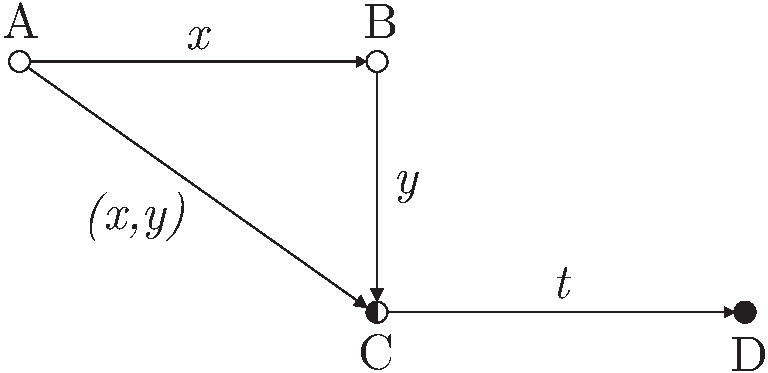
\includegraphics[width=0.7\textwidth]{files/methodeDerGeraden.pdf}
  \caption{Zwei verschiedene Möglichkeiten, zur semidiskreten Form C zu gelangen. Der Weg über B entspricht dabei der \emph{Methode der Geraden}. Im Punkt C verbleibt ein System gewöhnlicher DGLn, welches mit einem geeigneten Zeitschrittverfahren gelöst wird.}
  \label{fig:methodeDerGeraden}
\end{figure}
In Anbetracht der Randbedingungen aus Kapitel \ref{sec:RB} ist das Hybridverfahren ein intuitiverer Zugang, denn die Randbedingungen können nicht einfach als Dirichlet-Randbedingungen auf $\Gamma$ gesetzt werden. Stattdessen ist eine Unterscheidung hinsichtlich der Geschwindigkeit notwendig, was wiederum eine Diagonalisierung des Ableitungsoperators $\partial_y$ erfordert. Diese Diagonalisierung lässt sich mit der Methode der Geraden separieren von der $x$-Diskretisierung, vergleiche auch die Ausführungen in \cite{lukas1}. Die Diagonalisierung entspricht letztlich einer Fourier-Transformation (FT), denn im Impulsraum ist der Ableitungsoperator  diagonal. Eine \ac{dg}-Diskretisierung bzgl. $y$ hätte dabei jedoch zur Folge, dass die FT für \emph{double-valued}\footnote{An Kanten ist der Funktionswert nicht eindeutig definiert. Es gibt jeweils einen zu Element 1 und einen zu Element 2 zugehörigen Wert, siehe auch Abbildung \ref{fig:notation_DG}.} Punkte ausgewertet werden muss.

Eine weitere Motivation für das Hybridverfahren ist die Charakteristik der \ac{pdg} nach erfolgter $y$-Diskretisierung. Dann liegt nämlich ein System von Advektions-Reaktions-Gleichungen vor, was wiederum den Transportcharakter der \ac{pdg} offenbart. \ac{dg}-Verfahren sind wie bereits in Abschnitt \ref{sec:Übersicht} angesprochen dank einer flexiblen Wahl des numerischen Flusses für eben solche Transportgleichungen ausgelegt.

In einem vorbereitenden Einschub sollen im Folgenden einige wichtige Erkenntnisse aus der Theorie für Riemann Probleme hyperbolischer Systeme gezeigt werden. Sie werden später in Abschnitt \ref{sec:Hybridverfahren} benötigt, um einen korrekten numerischen Fluss zu formulieren.

\subsection{Riemann Probleme in hyperbolischen Systemen}\label{sec:riemann}\index{Riemann Problem}
Die folgenden Ausführungen orientieren sich an dem Buch von Leveque \cite{buchLeveque}.
Das Riemann Problem für die skalare Advektionsgleichung $u_t + f_x(u) = 0$ mit dem Fluss $f(u(x)) = s u(x)$ ist durch die diskontinuierliche Anfangswertbedingung
\begin{equation}
  u(x,0) = \begin{cases} u^- , \; x < 0 \\
                         u^+ , \; x > 0
           \end{cases}
\end{equation}
gestellt.  Die \emph{Rankine-Hugoniot-Bedingung}\index{Rankine-Hugoniot-Bedingung} lautet im skalaren Fall
\begin{equation}
  s(u^- - u^+) = (f^- - f^+) \; .
  \label{eq:rhc}
\end{equation}
Die Größe s ist dabei die Geschwindigkeit, mit der sich die Diskontinuität ausbreitet (\emph{shock speed}). Im allgemeineren Fall eines linearen Systems mit $f(u) = A u$ wird angenommen, dass die Matrix $A$ reelle, disjunkte Eigenwerte $\lambda_1 < \lambda_2 < \dots < \lambda_m$ hat, das heißt $A$ ist diagonalisierbar gemäß
\begin{equation}
  A = R \Lambda R^{-1}
\end{equation}
mit $R=[r_1 \, r_2 \, \dots \, r_m]$ als Transformationsmatrix mit den zugehörigen Eigenvektoren. Die Eigenwertgleichung lautet
\begin{equation}
  Ar_p = \lambda_p r_p \qquad \forall \, p=1,\dots, m
  \label{eq:EWeq_A}
\end{equation}
Durch die Zerlegung von $u^-$ und $u^+$ in die Eigenwertbasis gemäß
\begin{equation*}
  u^- = \sum_{p=1}^m \alpha_p r_p \qquad u^+ = \sum_{p=1}^m \beta_p r_p,
\end{equation*}
folgt mit $v = R^{-1}u$ und wegen der Charakteristik der Advektionsgleichung
\begin{equation*}
  v_p(x,t) = \begin{cases} \alpha_p , \; x - \lambda_p t < 0 \\
                           \beta_p  , \; x - \lambda_p t > 0
             \end{cases}
\end{equation*}
Bezeichnet $J(x,t)$ den größtmöglichen Index $p$, für den $x-\lambda_p t > 0$ gilt, so ist
\begin{align}
  u(x,t) = \sum_{p=1}^{J(x,t)} \beta_p r_p + \sum_{p={J(x,t)}+1}^m \alpha_p r_p \; .
\end{align}
Dieser Zusammenhang wird in Abbildung \ref{fig:torte} gezeigt.
\begin{figure}
  \centering
  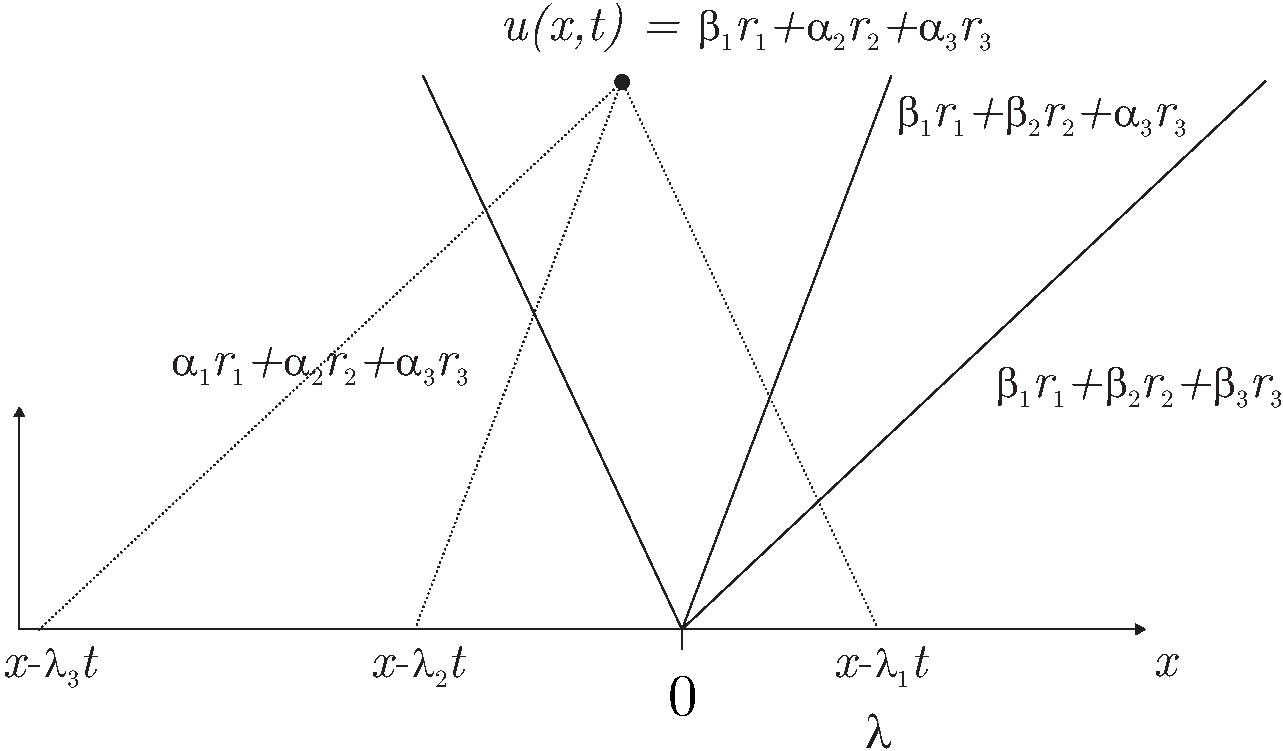
\includegraphics[width=0.7\textwidth]{files/Torte.pdf}
  \caption{Konstruktion der Lösung mit Hilfe der Charakteristiken-Methode am Beispiel dreier Eigenwerte $\lambda_1,\lambda_2,\lambda_3$. In den einzelnen Segmenten ist die Lösung konstant und ergibt sich als Linearkombination der Anfangswerte wie eingezeichnet.}
  \label{fig:torte}
\end{figure}
Die Lösung ist konstant innerhalb der einzelnen Segmente. Entlang der $p$-ten Charakteristik $x_p=\lambda_p t$ springt die Lösung jedoch. Mit der zu \ref{def:jump} äquivalenten Definition des Sprungs ${\jump{u}\equiv u^- - u^+}$ lässt sich
\begin{equation}
  -\jump{u_p} = (\beta_p - \alpha_p) r_p \; ,
  \label{eq:TortenJump}
\end{equation}
schreiben, wie der Abbildung zu entnehmen ist. Hier ist wieder die Rankine-Hugoniot-Bedingung analog zu Gleichung \eqref{eq:rhc} ersichtlich, denn es ist mit $f(u) = A u$
\begin{equation}
  \begin{aligned}
    \jump{f}_p &= A\jump{u}_p \stackrel{\eqref{eq:TortenJump}}{=} -(\beta_p - \alpha_p) A r_p \stackrel{\eqref{eq:EWeq_A}}{=}  -(\beta_p - \alpha_p) \lambda_p r_p \\
    &= \lambda_p \jump{u}_p \; .
  \end{aligned}
\end{equation}
Um nun den numerischen Fluss $\hat{f}$ eines \ac{dg}- oder \ac{fv}-Verfahrens zu bestimmen, ist $u$ an dem Ort $x=0$ auszuwerten (was in diesen Verfahren den Elementkanten entspricht). Daher können entweder von $u^-$ ausgehend die Sprünge nach rechts oder von $u^+$ ausgehend die Sprünge nach links aufaddiert  werden. Folglich gilt
\begin{align}
  \label{eq:rhc_1}
  u(x=0) &= u^- + \sum_{\lambda_p < 0} (\beta_p - \alpha_p)r_p = u^+ - \sum_{\lambda_p > 0} (\beta_p - \alpha_p)r_p \\
  \Rightarrow \qquad u(x=0) &= \frac{u^- + u^+}{2} + \frac{1}{2}\left( \sum_{\lambda_p < 0} (\beta_p - \alpha_p)r_p - \sum_{\lambda_p > 0} (\beta_p - \alpha_p)r_p \right) \; .
\end{align}
Multiplikation mit $A=R\Lambda R^{-1} = R(\Lambda^+ + \Lambda^-)R^{-1}$ (hierbei enthält $\Lambda^{+(-)}$ ausschließlich die positiven (negativen) Eigenwerte von $\Lambda$) ergibt den numerischen Fluss
\begin{align*}
  \hat{f} = A \avg{u} + \frac{1}{2}& (R(\Lambda^+ + \Lambda^-)R^{-1}) \sum_{\lambda_p < 0} (\beta_p - \alpha_p)r_p \\
                     - \frac{1}{2}& (R(\Lambda^+ + \Lambda^-)R^{-1}) \sum_{\lambda_p > 0} (\beta_p - \alpha_p)r_p \\
         = A \avg{u} + \frac{1}{2}&\left( R\Lambda^-R^{-1} \sum_{\lambda_p < 0} (\beta_p - \alpha_p)r_p
                    - R\Lambda^+R^{-1} \sum_{\lambda_p > 0} (\beta_p - \alpha_p)r_p        \right) \; .
\end{align*}
Die letzte Gleichheit folgt aus $\sum_j (R^{-1})_{i,j} (r_p)_j = \delta_{i,p} e_p$ (mit $e_p$ als Einheitsvektor). Im Folgenden soll mit $|A|$ die Kurzschreibweise für $(|A|)_{i,j} = |A_{i,j}|$ verwendet werden. Dann lässt sich der Fluss weiter zusammenfassen:
\begin{align}
  \hat{f} &= A \avg{u} + \frac{1}{2} \left( -R|\Lambda^-|R^{-1} \sum_{\lambda_p < 0} (\beta_p - \alpha_p)r_p
              - R\Lambda^+R^{-1} \sum_{\lambda_p > 0} (\beta_p - \alpha_p)r_p        \right) \\
        &= A \avg{u} - \frac{1}{2} \underbrace{(R|\Lambda^-|R^{-1} + R\Lambda^+R^{-1})}_{=R|\Lambda|R \equiv |A|}  \sum_p(\beta_p - \alpha_p)r_p   \\
        &\stackrel{\eqref{eq:rhc_1}}{=} A \avg{u} - \frac{1}{2} |A| (u^+-u^-) \\
        &= A \avg{u} + \frac{1}{2} |A| \jump{u} \; .
\end{align}
Die gesamte Argumentation funktioniert auch, wenn A bereits diagonal ist. Am Ausgangspunkt der vektoriellen Advektionsgleichung wird direkt eine Transformation $u=Rv$ durchgeführt, sodass
\begin{align}
  v_t + \Lambda v_x = 0 \; .
\end{align}
Es folgt dann wie oben gezeigt der numerische Fluss
\begin{align}
  \hat{f} = \hat{\Lambda v} = \Lambda\avg{v} + \frac{1}{2}|\Lambda|\jump{v} \; .
  \label{eq:FLUX}
\end{align}


\subsection{Hybridverfahren}\label{sec:Hybridverfahren}
In natürlichen Einheiten kann die bezüglich $y$ diskretisierte \ac{lvn} \eqref{eq:lvn} allgemein durch
\begin{equation}
  {A}^y u_t(x,t) + {B}^y u_x(x,t) + {C}^y(x,t)u(x,t) = 0
  \label{eq:qschema}
\end{equation}
geschrieben werden. Die Matrizen  ${A}^y$, ${B}^y$ und ${C}^y$ resultieren in diesem Abschnitt aus einem \ac{fv}-Verfahren, können aber ebenso anderen Verfahren entstammen.

Dem \ac{fv} Ansatz in \cite{lukas1} folgend wird das Intervall ${[-L_y/2,+L_y/2]}$ in $K_y$ Zellen unterteilt. Hieraus ergeben sich demnach $K_y+1$ Kanten
\begin{equation*}
  {y_{\nicefrac{1}{2}}, y_{\nicefrac{3}{2}}, \dots, y_{K_y + \nicefrac{1}{2}} = -L_y/2, -L_y/2+\Delta y_1,\dots,+L_y/2} \; .
\end{equation*}
Hierbei ist $\Delta y_i$ das Volumen der i-ten Zelle. Der Ansatz führt zu simplen Matrizen der Dimension ${K_y\times K_y}$ mit nicht verschwindenden Einträgen gemäß
\begin{equation}
  \begin{aligned}
  {A}^y_{i,i} &= \Delta y_i \\
  {B}^y_{i,i+1} &= -\frac{i}{2} \qquad
  {B}^y_{i+1, i} = +\frac{i}{2}  \\
  {C}^y_{i,i}(x,t) &= \mathrm{i} \frac{\Delta y_i}{4} (B(x, y_{i+\nicefrac{1}{2}},t) + B(x, y_{i-\nicefrac{1}{2}},t))  \\
  {C}^y_{i,i+1}(x,t) &= C^y_{i+1,i}(x,t) = \mathrm{i} \frac{\Delta y_i}{4} B(x, y_{i+\nicefrac{1}{2}},t)  \; .
  \end{aligned}
  \label{eq:ABC}
\end{equation}
Dieses Schema impliziert, dass $u(x,t)$ an den Kanten als Mittelwert von rechts- und linksseitiger Zelle angenommen wird. Des weiteren sind  homogene Dirichlet Randbedingungen angenommen, also ${u(x,y_{\nicefrac{1}{2}}, t) = u(x,y_{K_y+\nicefrac{1}{2}}, t) = 0}$.

Die Matrix $B^y$ kann analytisch diagonalisiert werden. Es ist ${B^y = R\Lambda^y R^{\dagger}}$ mit der Diagonalmatrix
\begin{equation}
  \Lambda^y_{m,n} = \cos\left(\frac{2\pi n}{K_y+1}\right)\delta_{m,n}   \qquad m,n = 1,\dots,K_y
  \label{eq:Lambda}
\end{equation}
und zugehörigen Eigenvektoren
\begin{equation}
  R_{m,n} = i^m \sin\left(\frac{mn\pi}{K_y +1} \right)   \qquad m,n = 1,\dots,K_y \; .
\end{equation}
Die Matrix $R$ ist unitär: $R^{-1} = R^{\dagger}$. Der Einfachheit halber wird nun $\Delta y_i = h_y$ konstant gesetzt, sodass
\begin{equation}
  (A^y)^{-1}B^y = h_y^{-1}R\Lambda^y R^{-1}
\end{equation}
gilt. Mit der unitären Transformation
\begin{equation}
  v(x,t) \equiv R^{\dagger}u(x,t) \label{eq:trafo_uv}
\end{equation}
sowie der Definition
\begin{equation}
  G(x,t) \equiv h_y^{-1} R^{\dagger}C^y(x,t)R
  \label{eq:G}
\end{equation}
folgt die diagonalisierte \ac{pdg}
\begin{equation}
  v_t(x,t) + \Lambda^y v_x(x,t) + G(x,t)v(x,t) = 0 \; .
  \label{eq:diagLVN}
\end{equation}
Dies ist ein System von $K_y$ gekoppelten Advektions-Reaktions-Gleichungen mit Anfangsbedingung
\begin{align}
  v(x,0) = (v(y_1,x,0),\dots,v(y_{K_y},x,0))^T = {v}_0(x) = R^{-1}u_0(x)
\end{align}
und Fluss ${{f}({v}(x,t))=\Lambda^y {v}(x,t)}$. Zur Formulierung der Randbedingungen gemäß den Überlegungen in Kapitel \ref{sec:RB} muss zunächst der Einströmrand $\Gamma^-$ definiert werden.
Sei dazu ${\Omega_x = (-L_x/2,L_x/2)}$ ein beschränktes, offenes Gebiet mit Lipschitz Rand $\partial\Omega_x$ in  $\mathbb{R}$. Es bezeichne $\Gamma_x\equiv (\partial\Omega_x)^{K_y}$ die Zusammenfassung des Randes der $K_y$ \ac{pdg}n. Der Einströmrand kann dann definiert werden gemäß
\begin{equation}
  \Gamma^- \equiv \{x\in\Gamma_x : \Lambda \cdot n(x) < 0\} \; ,
\end{equation}
wobei $n(x)$ der bzgl. $\Omega_x$ nach außen zeigende Normalenvektor ist. Um nun die Randbedingung aus Gleichung \eqref{eq:rb4} einzubringen, müssen diese gemäß Gleichung \eqref{eq:trafo_uv} noch transformiert werden. Es folgen die gesuchten Randbedingungen für das System \eqref{eq:diagLVN}:
\begin{equation}
  \begin{aligned}
    v(x,t) &= g(x,t) \qquad \text{auf }{\Gamma^-} \text{ mit} \\
    g(\nicefrac{x_r}{x_l},t) &= R^{\dagger} \left(\int \frac{\diff k}{2\pi} \cos(ky_1)     f_{\nicefrac{r}{l}} (k), \dots,
                                            \int \frac{\diff k}{2\pi} \cos(ky_{K_y}) f_{\nicefrac{r}{l}} (k)\right)^T
  \end{aligned}
\end{equation}
Das Gebiet $\Omega_x$ wird durch die Vereinigung von $K_x$ nicht überlappenden Elementen ${D^k = [x_{k-\nicefrac{1}{2}} , x_{k+\nicefrac{1}{2}}]}$ trianguliert und diese Triangulierung sei mit $\mathcal{T}$ bezeichnet. Gesucht wird eine diskrete Lösung $v\fin$ als Element des Finite-Elemente-Raumes
\begin{equation}
  X\fin = (X_{\mathcal{T},1})^{K_y} \equiv \left( \{ v \in L^1(\Omega_x) \; : \; v\rvert_{D^k} \in P_N(D^k) \, \forall \, k=1,\dots,K_x \} \right)^{K_y} \; ,
  \label{eq:FES}
\end{equation}
wobei $P_N$ der ${N+1=N_p}$ -dimensionale Raum der Polynome vom Grad $N$ ist. $X_{\mathcal{T},1}$ ist Teilmenge des gebrochenen Sobolev-Raumes
\begin{equation}
    H^1(\mathcal{T}) = \{ v \in L^2(\Omega_x) \; : \; v|_{D^k} \in H^1(D^k) \, \forall \, D^k \in \mathcal{T} \} \; ,
\end{equation}
welcher wiederum \underline{nicht} Teilmenge des Lösungsraumes $X=H^1(\Omega)$ ist. Dies zeigt die Nicht-Konformität der Methode. Dennoch ist auch $H^1(\mathcal{T})$ Hilbertraum und es lässt sich der Satz von Lax-Milgram anwenden.

Der finite Elemente Raum \eqref{eq:FES} lässt Unstetigkeiten zu und diese werden gemäß Abbildung \ref{fig:notation_DG} gekennzeichnet. Werte am linken Rand eines Elementes bekommen den Index "+" und Werte am rechten Rand den Index "-".
\begin{figure}
  \centering
  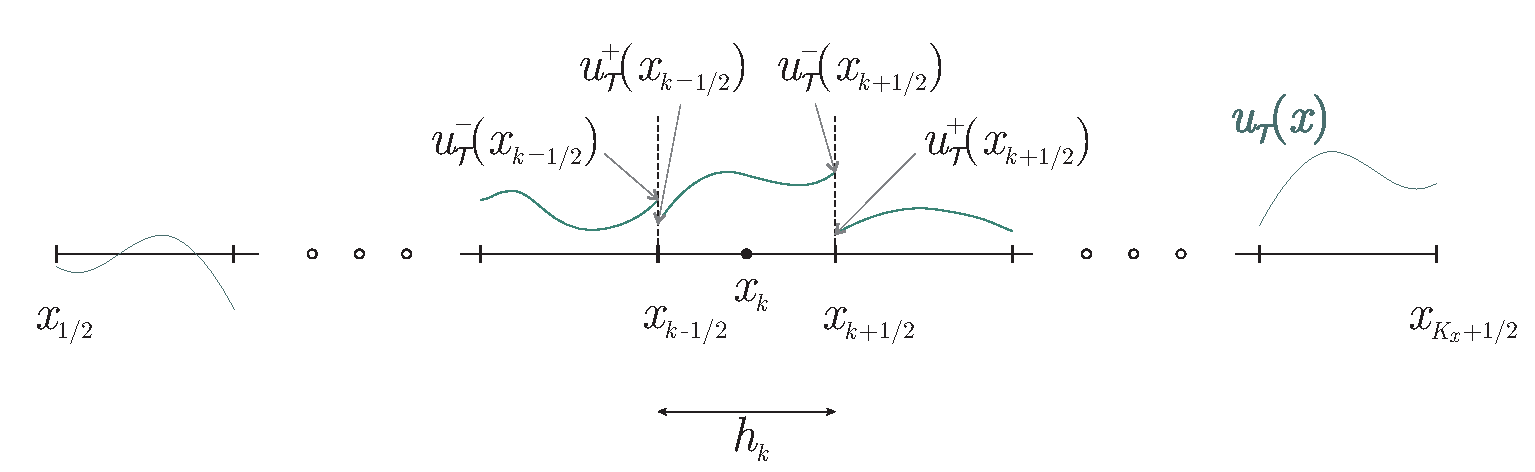
\includegraphics[width=0.95\textwidth]{files/notationDG.pdf}
  \caption{Notation für das eindimensionale \ac{dg}-Verfahren.}
  \label{fig:notation_DG}
\end{figure}
\begin{definition}[Sprung und Mittelwert]\label{def:jump}
Es bezeichne $F=\cup_{D^k\in\mathcal{T}} \, \partial D^k$ die Menge aller Elementkanten. Auf inneren Kanten $e\in F_i=F  \textbackslash \partial\Omega_x$ werden
\begin{equation}
  \jump{u\fin}_e = u\fin^-|_e - u\fin^+|_e \qquad \avg{u\fin}_e = \frac{1}{2} (u\fin^-|_e + u\fin^+|_e)
  \label{eq:jump_def_inner}
\end{equation}
als Sprung $\jump{u\fin}_e$ und Mittelwert $\avg{u\fin}_e$ von $u\fin \in X\fin$ definiert. Auf den zwei äußeren Kanten $e\in F_e = F \textbackslash F_i$ wird diese Definition durch
\begin{equation}
  \jump{u\fin}_e \equiv
        \begin{cases}
          -u_{\mathcal{T},l}^+ \equiv -u\fin(x_{\nicefrac{1}{2}})     \; \text{, links}\\
           u_{\mathcal{T},r}^- \equiv  u\fin(x_{K_x+\nicefrac{1}{2}}) \; \text{, rechts}
        \end{cases}
   \qquad \avg{u\fin}_e = \begin{cases} u_{\mathcal{T},l}^+ \; \text{, links}\\ u_{\mathcal{T},r}^- \; \text{, rechts}\\  \end{cases}
   \label{eq:jump_def_outer}
\end{equation}
erweitert. Ganz analog werden Sprung und Mittelwert für $u \in X_{\mathcal{T},1}$ definiert. Damit gilt für  $u,v\in X\fin$ die Relation
\begin{equation}
  \jump{u^{\dagger}v} = c(\jump{u}^{\dagger}\avg{v} + \avg{u}^{\dagger}\jump{v})
  \label{eq:jump_relation}
\end{equation}
mit $c=1$ für innere und $c=\nicefrac{1}{2}$ für äußere Kanten.
\end{definition}
Um nun das \ac{dg} Schema zu entwickeln, wird die Gleichung \eqref{eq:diagLVN} in die variationale Formulierung \eqref{eq:approx_varprob} gebracht. Gesucht sind Bilinearform $a$ und Linearform $\ell$, an die folgende Anforderungen gestellt werden:
\begin{itemize}
  \item \emph{Konsistenz}\index{Konsistenz}: Für die schwache Lösung $u\in H^1(\Omega)$ der \ac{lvn} und jede Funktion $v\in L^2(\Omega)$, die elementweise in $H^1(D^k)$ ist, gilt ${a\fin(u,v)=\ell\fin(v)}$.
  \item Beschränktheit und Koerzivität der Bilinearform nach Definition \ref{def:koerz}.
\end{itemize}
Der zweite Punkt ist diffizil und kann einzig durch eine gute Wahl des numerischen Flusses gewährleistet werden.
Konsistenz hingegen wird erreicht, indem zu der analytischen Form \eqref{eq:diagLVN} lediglich Sprungterme hinzugefügt werden, welche für die schwache Lösung $u\in H^1(\Omega)$ verschwinden. Der Grund hierfür liegt im zweiten Sobolevschen Einbettungssatz \cite{buchPietro}. Demnach bettet $W^{m,p}(\Omega)$ stetig in $C^{l,\alpha}(\overline{\Omega})$ ein, falls die Sobolev-Zahl ${\text{sob}(W^{m,p})\geq l+\alpha}$.
Insbesondere ist für $\Omega\in\mathbb{R}^1$ die Sobolevzahl $\text{sob}(H^1) = 1-\nicefrac{1}{2}$, weshalb $H^1$ stetig in $C^0$ einbettet. Für die schwache Lösung verschwinden also Sprungterme.

Multiplikation der diagonalisierten \ac{lvn} \eqref{eq:diagLVN} mit einer Testfunktion $\varphi\in X\fin$, Integration über ein Element $D^k$ und anschließende partielle Integration liefert
\begin{equation*}
  \int_{D^k} (\varphi^{\dagger} \partial_t v - (\partial_x \varphi^{\dagger}) f(v) + \varphi^{\dagger} G v) + \int_{\partial D^k}\hat{n}\varphi^{\dagger}f = 0
\end{equation*}
mit dem nach außen zeigenden Normalenvektor $\hat{n}$. Das Residuum ist also erneut bezüglich der $L^2$-Norm orthogonal zu allen Testfunktionen. Durch Summation über alle $K_x$ Elemente folgt
\begin{equation*}
  \sum_{D^k\in\mathcal{T}}\int_{D^k} (\varphi^{\dagger} \partial_t v - (\partial_x \varphi^{\dagger}) f(v) + \varphi^{\dagger} G v)
  + \sum_{e\in F_i}\int_{e}\jump{\varphi^{\dagger}f} + \sum_{e\in F_e}\int_e \jump{\varphi^{\dagger}f}  = 0 \; .
\end{equation*}
Nun wird Relation \eqref{eq:jump_relation} und die Stetigkeit der schwachen Lösung $v$ genutzt (${\jump{v}=\jump{f}=0}$).
\begin{equation}
  \sum_{D^k\in\mathcal{T}}\int_{D^k} (\varphi^{\dagger} \partial_t v - (\partial_x \varphi^{\dagger}) f(v) + \varphi^{\dagger} G v)
  + \sum_{e\in F_i}\int_{e}\jump{\varphi^{\dagger}} f + \sum_{e\in F_e}\int_e \jump{\varphi^{\dagger}} f  = 0
  \label{eq:kontinForm}
\end{equation}
An dieser Stelle wird die schwache Lösung $v$ durch ihre diskrete Ritz-Approximation $v\fin$ ersetzt. Dabei wird in dieser Arbeit diese Ansatzfunktion gemäß der variationalen Formulierung \eqref{eq:approx_varprob} aus demselben Raum wie die Testfunktion gesucht, was dem \emph{Galerkin-Ansatz}\index{Galerkin-Ansatz} entspricht. Das führt dazu, dass der Fluss $f\fin = f(v\fin)$ nicht mehr eindeutig definiert ist auf den Elementkanten. Er wird durch den \emph{single-valued} \emph{numerischen Fluss}\index{numerischer Fluss} $\hat{f}$ ersetzt. Dieser ergibt sich in sinnvoller Weise aus der Lösung des Riemann-Problems aus Abschnitt \ref{sec:riemann}, denn die Situation im \ac{dg}-Verfahren entspricht gerade einem solchen Problem. Die Elementkanten entsprechen den Orten der Diskontinuitäten und die Matrix $\Lambda$ enthält wie gefordert disjunkte Eigenwerte.
Aufgabe des numerischen Flusses ist es, die Randbedingungen in einer schwachen Weise einzubauen. So sollte beispielsweise für positive Geschwindigkeiten $\lambda_j$ (als Eigenwerte von $\Lambda$) am linken Rand
\begin{equation*}
  (\hat{f}(g, v^+))_j = \lambda_j g(x=-L_x/2)
\end{equation*}
gelten und damit dem Upwind Charakter der \ac{pdg} Rechnung getragen werden. Der numerische Fluss
\begin{equation}
  \begin{aligned}
    \hat{f} = \begin{cases}
    \Lambda\avg{v}_e + \frac{1}{2}|\Lambda|\jump{v}_e & e\in F_i \\
    \frac{1}{2}\Lambda(v^- + g) + \frac{1}{2}|\Lambda|(v^- - g)   & e=x_{K_x+\nicefrac{1}{2}} \\
    \frac{1}{2}\Lambda(v^+ + g) + \frac{1}{2}|\Lambda|(g - v^+)   & e=x_{\nicefrac{1}{2}}
  \end{cases}
  \end{aligned}
\end{equation}
aus dem vorherigen Abschnitt entspricht einem \emph{Upwind Fluss}\index{Upwind Fluss}. Dabei kann der letzte Term als Strafterm angesehen werden, der Sprünge der Lösung "bestraft". Allgemein ließe sich statt $|\Lambda|/2$ ein Faktor $\tau$ einfügen. Der Upwind Fluss ist zwar ein Spezialfall dieser allgemeineren Formulierung, numerische Experimente zeigen jedoch in Konsistenz mit den Ergebnissen in \cite{feistauer2004}, dass lediglich $\tau=|\Lambda|/2$ akzeptable Ergebnisse liefert. Das entspricht der Erwartung, denn der Upwind Fluss stellt wegen Erfüllung der Rankine-Hugoniot-Bedingung die beste Approximation an $f$ dar. Es gilt insbesondere für die schwache Lösung $\hat{f}(u,u)=f(u)$, wodurch die \emph{Konsistenz}\index{Konsistenz} des Verfahrens sichergestellt ist. Der Upwind Charakter des Flusses wird deutlich, wenn einzelne Eigenwerte $\lambda$ betrachtet werden. Ist beispielsweise $\lambda>0$, so folgt wie gefordert $\hat{f}=\lambda v^-$ auf inneren Kanten und am rechten Rand sowie $\hat{f}=\lambda g$ am linken Rand.

Einsetzen des numerischen Flusses in Gleichung \eqref{eq:kontinForm} zusammen mit dem Übergang zur Ritz-Approximation $v\fin$ ergibt die \emph{schwache Formulierung} des Hybridverfahrens:
\begin{problem}[Schwache variationale Formulierung der \ac{lvn}]\index{Schwache variationale Formulierung der LvNG}
  \label{prob:weak}
  Finde ein ${v\fin\in X\fin}$, sodass für alle $\varphi\in X\fin$ gilt $a\fin^w(v\fin, \varphi) + b\fin(v\fin, \varphi) = \ell\fin(\varphi)$. Hierin sind
  \begin{align}
    a\fin^w(v\fin, \varphi) = &\sum_{D^k\in\mathcal{T}}\int_{D^k} ( - (\partial_x \varphi^{\dagger}) f(v\fin) + \varphi^{\dagger} G v\fin) \nonumber \\
    &+ \sum_{e\in F_i}\int_{e}\jump{\varphi^{\dagger}} (\Lambda\avg{v} + \frac{1}{2}|\Lambda|\jump{v}) \\
    &+ \int_{e_r} \jump{\varphi^{\dagger}} \frac{1}{2}(\Lambda + |\Lambda|)\jump{v\fin}
    + \int_{e_l} \jump{\varphi^{\dagger}} \frac{1}{2}(-\Lambda + |\Lambda|)\jump{v\fin} \nonumber \\
    b\fin^w(v\fin, \varphi) = &\sum_{D^k\in\mathcal{T}}\int_{D^k} \varphi^{\dagger} \partial_t v\fin \\
    \ell\fin(\varphi)  = &-\int_{e_r} \jump{\varphi^{\dagger}} \frac{1}{2}(\Lambda - |\Lambda|)g
      -\int_{e_l} \jump{\varphi^{\dagger}} \frac{1}{2}(\Lambda + |\Lambda|)g
  \end{align}
  mit der Diagonalmatrix $\Lambda$ aus Gleichung \eqref{eq:Lambda}, dem Driftterm $G$ aus Gleichung \eqref{eq:G} sowie dem Fluss ${f(v)=\Lambda v}$.
\end{problem}
Integrale über Kanten dienen hier lediglich der Übersicht. Da sie aber im Eindimensionalen Auswertungen an einem Punkt entsprechen, sind sie letztlich redundant. Eine weitere partielle Integration des Flussterms führt auf die \emph{starke Formulierung}, die höhere Regularität an $u\fin$ fordert. Der dabei auftretende Term $\jump{\varphi^{\dagger}f(v\fin)}$ lässt sich mit Hilfe der Relation \eqref{eq:jump_relation} umformen.
\begin{problem}[Starke variationale Formulierung der \ac{lvn}]\index{Starke variationale Formulierung der LvNG}
  \label{prob:strong}
  Finde ein $v\fin\in X\fin$, sodass für alle $\varphi\in X\fin$ gilt $a\fin^s(v\fin, \varphi) + b\fin(v\fin, \varphi) = \ell\fin(\varphi)$. Hierin sind
  \begin{equation}
    \begin{aligned}
    a\fin^s(v\fin, \varphi) = &\sum_{D^k\in\mathcal{T}}\int_{D^k} (
    \varphi^{\dagger} \partial_x f(v\fin) + \varphi^{\dagger} G v\fin) \\
    &+ \sum_{e\in F_i}\int_{e}  (\jump{\varphi^{\dagger}} \frac{1}{2}|\Lambda| - \avg{\varphi^{\dagger}}\Lambda) \jump{v\fin} \\
    &+ \int_{e_r} \jump{\varphi^{\dagger}} \frac{1}{2}(-\Lambda + |\Lambda|)\jump{v\fin}
    + \int_{e_l} \jump{\varphi^{\dagger}} \frac{1}{2}(\Lambda + |\Lambda|)\jump{v\fin}
  \end{aligned}
  \label{eq:bilinear_strong}
  \end{equation}
  und $b,\ell$ wie in der schwachen Formulierung \ref{prob:weak} definiert.
\end{problem}

\subsection{Existenz und Eindeutigkeit}
Für die Bilinearform aus Problem \ref{prob:strong} soll im Folgenden die Existenz und Eindeutigkeit der Ritz-Approximation für die stationäre \ac{lvn} mit $\partial_t=0$ untersucht werden. Dazu ist Koerzivität nach Definition \ref{def:koerz} erforderlich. Es gilt mit $v\in X\fin$
\begin{align*}
  \sum_{D^k\in\mathcal{T}}\int_{D^k} v^{\dagger} \partial_x f(v) &=
  \frac{1}{2}\partial_x \sum_{D^k\in\mathcal{T}}\int_{D^k} v^{\dagger} f(v) \\
  &= \sum_{e\in F}\int_e \frac{1}{2}\jump{v^{\dagger} f(v)} \\
  &\stackrel{\eqref{eq:jump_relation}}{=}  \sum_{e\in F_i}\int_e \avg{v^{\dagger}} \jump{f(v)} + \sum_{e\in F_e}\int_{e} \frac{1}{2}\avg{v^{\dagger}} \jump{f(v)} \\
  &\stackrel{\eqref{eq:jump_def_outer}}{=} \sum_{e\in F_i}\int_e \avg{v^{\dagger}} \jump{f(v)} + \int_{e_r}\frac{1}{2} \jump{v^{\dagger}}\jump{f(v)} - \int_{e_l}\frac{1}{2} \jump{v^{\dagger}}\jump{f(v)} \; .
\end{align*}
Dieser Ausdruck hebt sich folgerichtig mit den entsprechenden Termen der Bilinearform \eqref{eq:bilinear_strong} auf. Es verbleibt
\begin{equation}
  \begin{aligned}
    a\fin^s(v, v) = &\sum_{D^k\in\mathcal{T}}\int_{D^k} v^{\dagger} G v
    + \sum_{e\in F}\int_e  \jump{v^{\dagger}} \frac{1}{2}|\Lambda| \jump{v} \; ,
  \end{aligned}
\end{equation}
anhand dessen Form zu erkennen ist, dass lediglich der durch den numerischen Fluss eingeführte Strafterm sowie der Potentialterm $G$ stabilisierend wirken. Um den Realteil der Bilinearform zu erhalten, wird dessen komplex Konjugiertes hinzu addiert.
\begin{equation}
  \begin{aligned}
    2\operatorname{Re} (a\fin^s(v, v)) = &\sum_{D^k\in\mathcal{T}}\int_{D^k} v^{\dagger} (G+G^{\dagger}) v
    + \sum_{e\in F}\int_e  \jump{v^{\dagger}} |\Lambda| \jump{v}
  \end{aligned}
  \label{eq:koerz_result}
\end{equation}
An dieser Stelle ist die Anfälligkeit des Verfahrens ersichtlich. Damit die rechte Seite auf eine Norm von $v$ zurückgeführt werden kann, müssen zwei Bedingungen erfüllt sein. Erstens muss $\forall i=1\dots K_y$ gelten $\lambda_i\neq 0$ genau wie bereits im Transfermatrix-Verfahren (vergleiche Abschnitt \ref{sec:TFmethod}). Zweitens muss der Realteil aller Eigenwerte von $(G+G^{\dagger})$ gemäß der Bedingung \eqref{eq:koerz_imag} größer 0 sein. Gibt es solche Schranken $g_0$ und $\lambda_{\text{min}}$(als betragsmäßig kleinster Eigenwert von $\Lambda$), so folgt unmittelbar
\begin{align}
  \operatorname{Re}(a\fin^s(v, v)) \geq g_0 |||v||| \qquad \text{mit} \\
  \trinorm{.} = \sum_{D^k\in\mathcal{T}}\int_{D^k} |.|^2 + \sum_{e\in F}\int_e  \frac{\lambda_{\text{min}}}{g_0} |\jump{.}|^2 \; . \label{eq:trinorm}
\end{align}
Andernfalls ist die Bilinearform nicht koerzitiv. Dieses Resultat ist konsistent mit den Erkenntnissen in der Literatur \cite{feistauer2007}, wo das skalare Problem
\begin{equation*}
  \partial_t u + \vec{v}\cdot \nabla u - \epsilon\Delta u + cu = g
\end{equation*}
mit einem elliptischen Anteil $\propto \epsilon$ betrachtet wird. Die Koerzivität der Bilinearform beruht für $\epsilon=0$ dort auf der Annahme, dass ${c-\nicefrac{1}{2}\,\text{div}\,\vec{v}\geq \gamma_0 > 0 \, \forall x\in\Omega_x}$ gilt. Im Fall der diagonalisierten \ac{lvn} entspricht die Geschwindigkeit $\vec{v}$ den Eigenwerten $\Lambda$, deren Ableitung wegen der expliziten Form \eqref{eq:Lambda} verschwindet.

Das Eigenwertspektrum von $G(x)+G^{\dagger}(x)$ gleicht dem Spektrum von $C(x)+C^{\dagger}(x)$ (modulo Faktor $h_y>0$), da $C$ und $G$ über die unitäre Transformation \eqref{eq:G} miteinander verknüpft sind. Die Matrix $C$ ist nach Gleichung \eqref{eq:ABC} symmetrisch, weshalb $C+C^{\dagger}=2\operatorname{Re}(C)$ gelten muss. Anhand Gleichung \eqref{eq:cap} ist zu sehen, dass der Realteil von $C$ einzig aus dem \ac{cap} besteht.
Offenbar ist $\operatorname{Re}(C)$ positiv semidefinit, da $W_0<0$ gilt. Die untere Schranke $g_0$ entspricht also leider gerade $0$. Koerzivität nach Definition \ref{def:koerz} und damit einhergehend Existenz der Ritz-Approximation für das Problem \ref{prob:strong} ist somit nicht gewährleistet. Interessant ist, dass dieses Resultat in Einklang mit den in Kapitel \ref{sec:RB} beschriebenen Überlegungen zur Nicht-Eindeutigkeit der stationären Lösung steht.

Es ist anzumerken, dass die Wahl des numerischen Flusses keinerlei Einfluss auf den Volumenteil der Norm in \eqref{eq:trinorm} hat. Schließlich können bestenfalls Sprungterme  ergänzt werden, die jedoch beispielsweise für $v\in C^0(\Omega)$ verschwinden und somit auch nicht mit einer eventuellen Spurungleichung in den Volumenteil der Norm eingehen können. Dies scheint ein inhärentes Problem zu sein.

% Aus Koerzivität folgt  Eindeutigkeit der Lösung, denn angenommen es gebe zwei Lösungen $v\fin^1$ und $v\fin^2$. Dann gilt $a\fin^s(v\fin^1-v\fin^2,\varphi)=0$ und mit der Wahl ${\varphi=v\fin^1-v\fin^2}$ folgt aufgrund der Koerzivität $0\geq g_0 \trinorm{v\fin^1-v\fin^2}$ und somit $v\fin^1=v\fin^2$. Im endlich-dimensionalen folgt aus der Eindeutigkeit die Existenz. Alternativ ließe sich auch die Beschränktheit der Bilinearform und dann mit Satz \ref{laxmilgram} die Existenz zeigen.

Auffällig an der Argumentation ist, dass die Randbedingungen lediglich in Form ihrer Charakteristik zur Definition eines Upwind Flusses eingehen. Solange die rechte Seite des Variationsproblems $\ell(\varphi)$ in $\mathcal{L}(X\fin,\mathbb{C})$ liegt, ist die konkrete Form von $g(x)$ nicht weiter relevant.

\subsection{Stabilität}\label{sec:stabilität}
Stabile Lösungen zeichnen sich dadurch aus, dass alle Eigenwerte des Liouvilleoperators aus Gleichung \eqref{eq:Liouvilleoperator} negativen Imaginärteil haben, wie sich leicht anhand der Form $i\td{}{t}\rho = \mathcal{L}\rho$ nachvollziehen lässt. Numerisch kann einerseits das Eigenwertspektrum der entsprechenden Matrix untersucht werden. Andererseits kann und soll im Folgenden eine Abschätzung für den Term $\td{}{t}\norm{v\fin}_{L^2(\Omega_x)}^2$ gefunden werden. Dazu wird zu der starken Formulierung \ref{prob:strong} ihr komplex konjugiertes hinzu addiert und die Testfunktion $\varphi=v\fin$ verwendet. Mit Hilfe des Resultates \eqref{eq:koerz_result} für den stationären Anteil der Bilinearform sowie den Überlegungen bezüglich des Driftterms aus dem vorherigen Abschnittes folgt
\begin{align}
  \td{}{t}\norm{v\fin}_{L^2(\Omega_x)}^2
  &= - \sum_{D^k \in \mathcal{T}} \int_{D^k} v\fin^{\dagger}(G+G^{\dagger})v\fin
  - \sum_{e\in F}\int_e  \jump{v^{\dagger}} |\Lambda| \jump{v\fin}
  + 2\operatorname{Re}(\ell\fin(v\fin)) \nonumber \\
 &\stackrel{g_0=0}{\leq} -  \sum_{e\in F}\int_e \lambda_{\text{min}}  |\jump{v\fin}|^2
       + 2\operatorname{Re}(\ell\fin(v\fin)) \label{eq:stabi} \; .
\end{align}
Mit der Annahme $-  \sum_{e\in F}\int_e \lambda_{\text{min}}  |\jump{v\fin}|^2  \leq 2\operatorname{Re}(\ell\fin(v\fin))$ folgt die Stabilität. Diese Behauptung wiederum soll in der vorliegenden Arbeit lediglich \emph{a posteriori} bestätigt werden. Sie lässt sich \emph{hand-wavy} dadurch begründen, dass die Randbedingungen symmetrisch sind und die approximierende Lösung $v\fin$ für hinreichend große $L_x$ keine großen Sprünge gegenüber der Fermi-Dirac-Statistik $g(x)$ zeigt. Damit heben sich die beiden in $\ell$ enthaltenen Terme am linken und rechten Rand in etwa auf.
Numerische Experimente zeigen, dass ein Abweichen vom Upwind Fluss mit dem Strafparameter $\tau=|\Lambda|/2$ hin zu kleineren $\tau$ zur Instabilität des transienten Systems führen. Da $\tau$ unmittelbar mit $\lambda_{\text{min}}$ korreliert, ist dies ein weiteres Indiz für die Gültigkeit der Ungleichung \eqref{eq:stabi} sowie der getroffenen Annahme.

Eine ähnliche Stabilitätsanalyse wird in der Literatur \cite{NLS} vorgenommen mit dem entscheidenden Unterschied, dass dort periodische Randbedingungen angenommen werden, sodass sich die beiden Terme tatsächlich exakt aufheben.

Zusammenfassend bleibt respektive der Ungleichung \eqref{eq:stabi} die wichtige Erkenntnis, dass zwei Faktoren die Stabilität des Verfahrens ermöglichen. Dies sind erstens der Strafterm $|\Lambda|/2\jump{v}$ des numerischen Flusses und zweitens das \ac{cap} aus Abschnitt \ref{sec:RB}.

\subsection{Implementierung}
Die Implementierung richtet sich in wesentlichen Zügen an der Ausarbeitung des dritten Kapitels des eingangs erwähnten Buches \cite{buch}. Im Folgenden werden die wichtigsten Punkte zusammengefasst. Das \ac{dg}-Verfahren wird dabei der Einfachheit halber zunächst als eindimensional angesehen mit $v\fin \in X_{\mathcal{T},1}$. An relevanten Stellen wird die Einbettung in das System mit $v\fin \in X\fin$ berücksichtigt, vergleiche Gleichung \eqref{eq:FES}.

Die Ritz-Approximation $v\fin \in X_{\mathcal{T},1}$ ist lokal definiert. \emph{Lokal}\index{lokale Darstellung der Ritz-Approximation} bedeutet hier stets eine elementweise Betrachtung für jedes Element $D^k$. Wie in jedem \ac{fem}-Verfahren überführt die affine Abbildung
\begin{equation}
  x\in D^k : \qquad x(r) = x_{k-\nicefrac{1}{2}} + \frac{1+r}{2}h_k, \qquad h_k=x_{k+\nicefrac{1}{2}} - x_{k-\nicefrac{1}{2}}
  \label{eq:affmap}
\end{equation}
die lokalen Integrale auf ein Referenzelement $I=[-1,1]$ mit $r\in I$.
Es wird dann zwischen \emph{modaler Darstellung}\index{modale Darstellung}
\begin{align}
  x\in D^k : \qquad v\fin^k(x(r),t) = \sum_{n=1}^{N_p}\hat{v}_{\mathcal{T},n}^k(t) \Psi_n(r)
\end{align}
und \emph{nodaler Darstellung}\index{nodale Darstellung}
\begin{align}
  x\in D^k : \qquad v\fin^k(x(r),t) = \sum_{i=1}^{N_p} v_{\mathcal{T},i}^k(t)\ell_i(r)
  \label{eq:nodal}
\end{align}
der Ritz-Approximation unterschieden. Dabei sind $\Psi_n(r)$ bzw. $\ell_i(r)$ verschiedene Basisfunktionen des Polynomraumes $P_N(I)$ (siehe auch Gleichung \eqref{eq:FES}). Für das System hat $v\fin^k(x,t)$ gerade $K_y$ Komponenten. Die entsprechenden Koeffizienten bekommen dann einen weiteren Index $v_{\mathcal{T},i}^k \rightarrow v_{\mathcal{T},i}^{k,j}$ mit $j=1,\dots,K_y$.

Die nodale Darstellung bietet den Vorteil, dass die Funktion nicht unbedingt ausgewertet werden muss, da $v\fin^k(x(\xi_i),t)$ durch die Entwicklungskoeffizienten $v_{\mathcal{T},i}^k(t)$ bereits gegeben ist. Es handelt sich hierbei also um eine interpolatorische Darstellung.
Eine hierfür geeignete Basis sind die Lagrange-Polynome
\begin{align}
  \ell_i(r) = \prod_{\substack{j=1 \\ j\neq i}}^{N_p} \frac{r-\xi_j}{\xi_i-\xi_j}
\end{align}
mit $N_p$ verschiedenen Knotenpunkten $\xi_j\in[-1,1]$ und der Eigenschaft ${\ell_i(\xi_j)=\delta_{ij}}$. Für eine Verallgemeinerung in höherdimensionale Probleme bietet es sich an, die benötigten Integrale über die Basisfunktionen mit Hilfe der modalen Basis $\Psi$ zu kalkulieren, da die Lagrange-Polynome sich nicht auf einfache Weise formulieren lassen. Für diese modale Basis wird für eine gute Konditionierung der Massenmatrix (vergleiche Gleichung \eqref{eq:Mmatrix}) statt der Monombasis die orthonormierte Basis
\begin{align}
  \Psi_n(r) = \frac{P_{n-1}(r)}{\sqrt{2(2n+1)^{-1}}}
  \label{eq:modaleBasis}
\end{align}
mit den Legendre Polynomen $P_n(r)$ gewählt. Der Zusammenhang zwischen nodaler und modaler Basis ist durch die \emph{Vandermonde-Matrix}\index{Vandermonde-Matrix}
\begin{equation}
  \begin{aligned}
    \van_{ij} = \Psi_j(\xi_i)
  \end{aligned}
  \label{eq:vandermonde}
\end{equation}
gegeben. Es gilt dann
  \begin{align}
    &\van\hat{v}\fin = v\fin        & &\text{sowie} \label{eq:nodalmodal}\\
    &\van^T\ell(r) = \Psi(r) & &\text{mit} \label{eq:ellPsi}\\
    &\hat{v}\fin = (\hat{v}_{\mathcal{T},1} \dots \hat{v}_{\mathcal{T},N_p})^T, & & v =(v_{\mathcal{T},1} \dots v_{\mathcal{T},N_p})^T \nonumber \\
    &\ell(r) = (\ell_1(r) \dots \ell_{N_p}(r))^T, & & \Psi(r) =(\Psi_1(r) \dots \Psi_{N_p}(r))^T \nonumber \; ,
  \end{align}
wobei der Index $\mathcal{T}$ der Übersicht halber temporär unterdrückt worden ist. Der Zusammenhang gilt wegen der affinen Abbildung \eqref{eq:affmap} für alle Elemente $D^k$, weshalb auch dieser Index unterdrückt worden ist.

Die Interpolationspunkte $\xi_j$ werden derart gewählt, dass die Interpolation möglichst nahe an der bestmöglichen Ritz-Approximation durch ein (allgemeines) Polynom liegt. Dies führt auf die Legendre-Gauß-Lobatto Quadraturpunkte. Besonders für hohe Polynomgrade $N\geq 5$ ist diese Wahl zu favorisieren, denn äquidistante Knoten würden hier zu einer exponentiell schlecht konditionierten Interpolation führen. Ein weiterer Vorteil offenbart sich, wenn für die spätere Fehlerberechnung die Funktion über $\Omega$ integriert werden muss. Hier bietet sich dann die Gauß-Lobatto-Quadratur an, sodass die Funktionsauswertung nach Gleichung \eqref{eq:nodal} entfällt, da lediglich $v\fin(\xi_j)$ benötigt wird und diese Funktionswerte gerade den Koeffizienten entsprechen.

Mit diesen Vorarbeiten kann nun die starke Formulierung \ref{prob:strong} in eine Matrix-Vektor-Gleichung überführt werden. Die Forderung der Gültigkeit für alle Testfunktionen $\varphi\in X_{\mathcal{T},1}$ übersetzt sich für einen $N_p$-dimensionalen Polynomraum in exakt $N_p \times K_x$ Gleichungen. Für das gesamte System mit $K_y$ Zellen in $y$-Richtung müssen sich entsprechend $N_p \times K_x \times K_y$ Gleichungen ergeben. Dazu wird lokal als Testfunktion $\varphi = \ell_m e_j$ gewählt mit dem Einheitsvektor $e_j$, wobei $m=1\dots N_p$ und $j=1\dots K_y$. Für die weitere Notation sowie die Implementierung dient die folgende Definition.
\begin{definition}[Massen- und Steifigkeits- und Driftmatrix, Notation der Lösung]\index{Massematrix}\index{Steifigkeitsmatrix}\index{Driftmatrix} \label{def:matrizen}
  Für die nodale Darstellung heißen
  \begin{equation*}
    (M^k)_{pq} \equiv \int_{x_{k-\nicefrac{1}{2}}}^{x_{k+\nicefrac{1}{2}}} \ell_p^k(x) \ell_q^k(x) \diff x = \frac{h_k}{2}\int_{-1}^1 \ell_p(r) \ell_q(r) \diff r \equiv \frac{h_k}{2} M_{pq}
    \label{eq:Mmatrix}
  \end{equation*}
  Massenmatrix,
  \begin{equation*}
    (S^k)_{pq} \equiv \int_{x_{k-\nicefrac{1}{2}}}^{x_{k+\nicefrac{1}{2}}} \ell_p^k(x) \td{\ell_q^k(x)}{x} \diff x = \int_{-1}^1 \ell_p(r) \td{\ell_q(r)}{r}  \diff r \equiv S_{pq}
    \label{eq:Smatrix}
  \end{equation*}
  Steifigkeitsmatrix und
  \begin{equation*}
    (\drift^{k,jm})_{pq} = \int_{D^k} G_{jm}(x) \ell_p^k(x) \ell_q^k(x) \diff x \qquad \forall j,m=1\dots K_y % v_{\mathcal{T},p}^{k,m} wird dadran multipliziert
  \end{equation*}
  Driftmatrix. Dabei ist $G_{jm}(x)$ die Matrixkomponente von $G(x)$ aus Gleichung \eqref{eq:G}. Hier und im Folgenden ist die explizite Zeitabhängigkeit temporär unterdrückt worden. Die nodalen Entwicklungskoeffizienten der Lösung des Variationsproblems $v\fin$ werden gemäß
  \begin{equation*}
    \begin{aligned}
      \underline{v} &= (\underline{v}_1 \dots \underline{v}_{K_y})^T        &  &\text{mit} \\
      \underline{v}_j &= (\underline{v}_j^1 \dots \underline{v}_j^{K_x})^T  &  &\text{mit} \\
      \underline{v}_j^k &= (v_{\mathcal{T},1}^{k,j} \dots v_{\mathcal{T},N_p}^{k,j})^T
    \end{aligned}
  \end{equation*}
  notiert und somit in einem globalen Vektor $\underline{v} \in \mathbb{C}^{s}$ mit $s=K_y K_x N_p$ zusammengefasst.
\end{definition}
Genau wie die bereits für das System definierte Driftmatrix lassen sich auch $M$ und $S$ für das System definieren. Sie sind bezüglich der $y$-Richtung blockdiagonal gemäß $(\mathcal{M}^{k,jm})_{pq} = \delta_{jm}(M^k)_{pq}$ und $\mathcal{S}$ analog.
Die eingeführten Matrizen lassen sich durch die Vandermondematrix $\van$ ausdrücken. Die Zusammenhänge für Massen- und Steifigkeitsmatrix sind durch
\begin{align*}
  M &= (\van\van^T)^{-1} \\
  M^{-1}S &= \van_r \van^{-1} \qquad \text{mit } (\van_r)_{ij} = \td{\Psi_j}{r}\biggr\rvert_{\xi_i}
\end{align*}
gegeben, wobei im Wesentlichen die Orthonormiertheit der gewählten modalen Basis \eqref{eq:modaleBasis} eingegangen ist. Für die Driftmatrix wird im Anhang \ref{sec:A_5} ein entsprechender Ausdruck hergeleitet. Es ist hierzu anzumerken, dass die Driftmatrix die einzige Kopplung bezüglich $y$-Richtung darstellt. Daher geht die Herleitung über eine eindimensionale Betrachtung des \ac{dg}-Verfahrens und damit über die Ausführungen in \cite{buch} hinaus.

Prinzipiell gibt es verschiedene Möglichkeiten, den Driftterm zu behandeln. Da jedoch Funktionswerte Von Ansatz- und Testfunktion bereits an den Gauß-Lobatto Quadraturpunkten vorliegen, bietet es sich an, diese Quadratur zu verwenden. Es wird im folgenden zwischen zwei Methoden unterschieden.
\begin{enumerate}
  \item (Methode G1) Es lässt sich von vornherein das Produkt $G(x)v\fin(x)$ in der nodalen Basis entwickeln. Dann ergibt sich für das resultierende Integral wieder die Massenmatrix. In dem lokalen Schema verbleibt dann nach Multiplikation mit $(M^k)^{-1}$ schlicht der Ausdruck ${\sum_{m=1}^{K_y}\text{diag}(\underline{G}^k_{jm})\underline{v}_m^k}$. Die Driftmatrix aus Definition \ref{def:matrizen} findet hierbei nicht Verwendung.
  \item (Methode G2) Eine genauere Betrachtung belässt $G(x)$ als analytisch bekannt, sodass die Driftmatrix mit Hilfe von Gauß-Lobatto-Quadratur höherer Ordnung berechnet werden kann. Mit der Quadraturordnung $N_{GL}$ ergibt sich mit den dem Anhang \ref{sec:A_5} zu entnehmenden Definitionen der Matrix $W$ und der Gewichte $w$
  \begin{equation}
    (\drift^{k,jm})_{pq} = \sum_{a=1}^{N_{GL}} W_{ap} W_{ai} w_a G_{jm}(\xi_a^k)\frac{h_k}{2} \; .
    \label{eq:G_GL}
  \end{equation}
  Diese Methode ist insbesondere für unstetige Potentiale wie das Flachbandpotential in Abbildung \ref{fig:pot1} zu bevorzugen, da solche Unstetigkeiten besser durch Polynome höherer Ordnung approximiert werden.
\end{enumerate}
Beide Ansätze sind numerisch anhand der resultierenden iterativen Fehler verglichen worden, siehe Kapitel \todo{ref}. Es zeigt sich erwartungsgemäß, dass der zweite Ansatz zu besseren Konvergenzraten führt. Offensichtlich ist dies aber gleichzeitig die rechenintensivere Option.

Nun lässt sich das Variationsproblem \ref{prob:strong} zunächst für festen Index $j$ und innere Elemente lokal umschreiben gemäß
\begin{equation}
  \begin{aligned}
    \forall D^k\in\mathcal{T} \textbackslash &\{D^1,D^{K_x}\} : \\
      &\partial_t \underline{v}_j^k + (M^k)^{-1}S \underline{f}_j^k + \sum_{m=1}^{K_y} (M^k)^{-1}\drift^{k,jm}\underline{v}_m^k \\
      &+ \left(\frac{-\lambda_j + |\lambda_j|}{2}\right) \jump{\underline{v}_j}_{e_r}\underline{E_r} +
         \left(\frac{-\lambda_j - |\lambda_j|}{2}\right) \jump{\underline{v}_j}_{e_l}\underline{E_l} = 0
  \end{aligned}
  \label{eq:schema1}
\end{equation}
wobei die lokalen \emph{Liftoperatoren}\index{Liftoperator}
\begin{equation}
  \begin{aligned}
    \underline{E_r} &\equiv (M^k)^{-1}\underline{\ell}(x_{k+\nicefrac{1}{2}}) = (M^k)^{-1}  \cdot (0,\dots,0,1)^T \\
    \underline{E_l} &\equiv (M^k)^{-1}\underline{\ell}(x_{k-\nicefrac{1}{2}}) = (M^k)^{-1}  \cdot (1,0,\dots,0)^T
  \end{aligned}
\end{equation}
eingeführt worden sind. Die letzte Gleichheit ergibt sich für Polynomgrade $N\geq{1}$, da ${ \{x_{k-\nicefrac{1}{2}}, x_{k+\nicefrac{1}{2}}\} = \{\xi_1, \xi_{N^p} \} }$ für die gewählten Gauß-Lobatto Quadraturpunkte. Der Sprung der Koeffizienten ist etwas fahrlässig notiert, um die Situation nicht unnötig unleserlich zu gestalten. Es ist für innere Kanten
\begin{align*}
  \jump{\underline{v}_j}_{e_r} &= v_{\mathcal{T},N_p}^{k,j} - v_{\mathcal{T},1}^{k+1,j} \qquad \text{und} \\
  \jump{\underline{v}_j}_{e_l} &= v_{\mathcal{T},1}^{k,j} - v_{\mathcal{T},N_p}^{k-1,j}
\end{align*}
gesetzt worden gemäß der Definition \eqref{eq:jump_def_inner}. Dieser Ausdruck entspricht wegen der interpolatorischen Eigenschaft der Lagrange-Polynome exakt dem Sprung der Ritz-Approximation. Die Zusammenhänge werden in Abbildung \ref{fig:notationDG2} veranschaulicht.
\begin{figure}
  \centering
  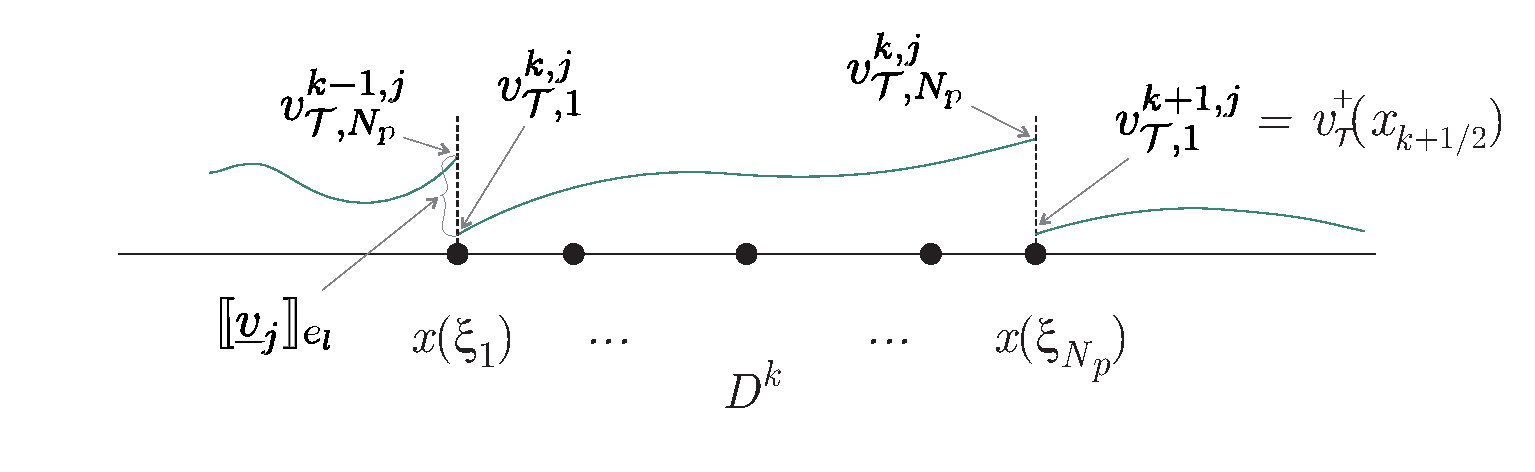
\includegraphics[width=0.95\textwidth]{files/notationDG2.pdf}
  \caption{Notation der nodalen Darstellung für das eindimensionale \ac{dg}-Verfahren. An den Knotenpunkten entspricht der Funktionswert gerade den Entwicklungskoeffizienten. Da für Gauß-Lobatto Knoten mit $N_p\geq 2$ stets $\xi_1=-1$ und $\xi_{N_p}=1$ gilt, entspricht der Sprung von $v\fin$ dem Sprung der Koeffizienten.}
  \label{fig:notationDG2}
\end{figure}
Für die beiden Randelemente ergibt sich
\begin{equation}
  \begin{aligned}
      &\partial_t \underline{v}_j^{K_x} + (M^{K_x})^{-1}S \underline{f}_j^{K_x} + \sum_{m=1}^{K_y} (M^{K_x})^{-1}\drift^{k,jm}\underline{v}_m^{K_x} \\
      &+ \left(\frac{-\lambda_j + |\lambda_j|}{2}\right) v_{\mathcal{T},N_p}^{K_x,j} \underline{E_r} +
         \left(\frac{-\lambda_j - |\lambda_j|}{2}\right) \jump{\underline{v}_j}_{e_l}\underline{E_l} =
         \left(\frac{-\lambda_j + |\lambda_j|}{2}\right) g_j(x_r,t)\underline{E_r}
  \end{aligned}
  \label{eq:schema2}
\end{equation}
\begin{equation}
  \begin{aligned}
      &\partial_t \underline{v}_j^{1} + (M^{1})^{-1}S \underline{f}_j^{1} + \sum_{m=1}^{K_y} (M^{1})^{-1}\drift^{k,jm}\underline{v}_m^{1} \\
        &+ \left(\frac{-\lambda_j + |\lambda_j|}{2}\right) \jump{\underline{v}_j}_{e_r}\underline{E_r} +
           \left(\frac{\lambda_j + |\lambda_j|}{2}\right) v_{\mathcal{T},1}^{1,j} \underline{E_l}
        =\left(\frac{\lambda_j + |\lambda_j|}{2}\right) g_j(x_l,t)\underline{E_l} \; .
  \end{aligned}
  \label{eq:schema3}
\end{equation}
Die Gleichungen \eqref{eq:schema1,eq:schema2, eq:schema3} werden in stationärer Form (das heißt $\partial_t \underline{v}=0$) als globales Matrix-Vektor-System implementiert, sodass das lineare Gleichungssystem
\begin{equation}
  \underline{\underline{\mathcal{A}}}\,\underline{v} = \underline{b}
  \label{eq:stat_LGS}
\end{equation}
resultiert mit der Systemmatrix $\underline{\underline{\mathcal{A}}}$ sowie dem Vektor $\underline{b}$, der sich aus der rechten Seite von \eqref{eq:schema2, eq:schema3} ergibt und die Randbedingungen enthält. Zur Lösung des LGS wird die \mat-interne Methode verwendet. Die gesuchte stationäre Dichtematrix ergibt sich schließlich aus der Rücktransformation \eqref{eq:trafo_uv}. Für die Zeitentwicklung wird dann ein explizites Zeitschrittverfahren angewandt, siehe Abschnitt \ref{sec:timestepping}.

Die Bestandteile der Systemmatrix werden in den folgenden Abbildungen für die Systemgröße $\{K_x=3, N_p=3, K_y=4\}$ exemplarisch gezeigt. Sie unterteilt sich in den Diffusionsterm $(M^k)^{-1}S\Lambda$, den Driftterm $(M^k)^{-1}\mathcal{G}^k$ sowie den Flussterm, welcher die Kantenterme beinhaltet. Die Abbildungen sind zur Verbesserung der Lesbarkeit mit einer farblichen Struktur unterlegt. Dabei ist Definition \ref{def:matrizen} hilfreich. Die grünen Rahmen bedeuten fixierte $y$-Diskretisierung (Indizes $j,m$ konstant). Die grauen Quadrate beranden ein Element der $x$-Diskretisierung ($D^k$ konstant), worin wiederum die $N_p \times N_p$ lokal definierten Matrizen $M^k$, $S^k$ und $\mathcal{G}^{k,jm}$ zu sehen sind.

Abbildung \ref{fig:matrix_L} zeigt den Diffusionsterm.
\begin{figure*}
    \centering
    \begin{subfigure}[b]{0.475\textwidth}
        \centering
        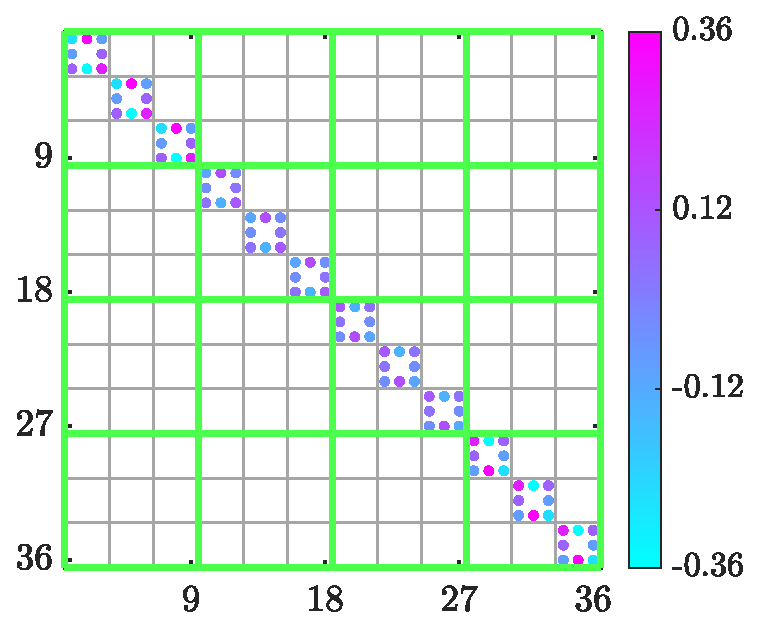
\includegraphics[width=\textwidth]{plots/L_glob.eps}
        \caption[]%
        {{\small Diffusionsmatrix}}
        \label{fig:matrix_L}
    \end{subfigure}
    \hfill
    \begin{subfigure}[b]{0.475\textwidth}
        \centering
        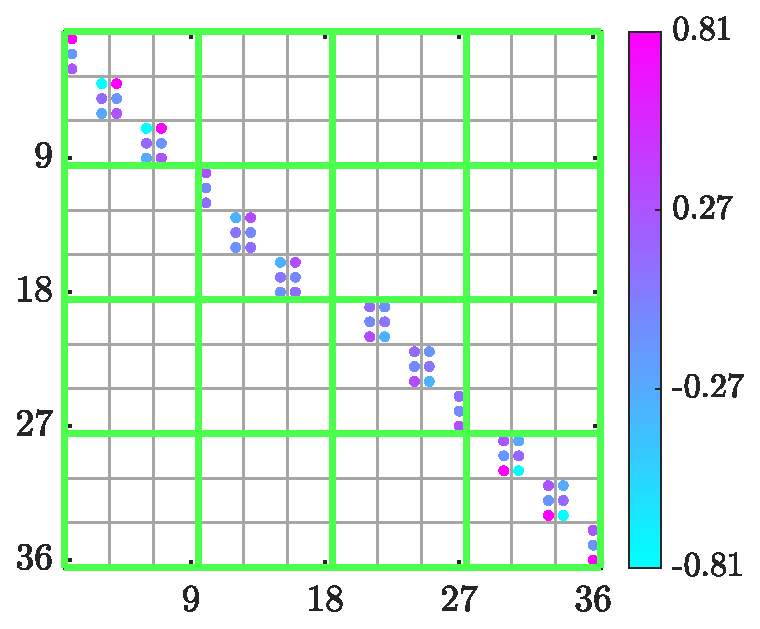
\includegraphics[width=\textwidth]{plots/F_glob.eps}
        \caption[]%
        {{\small Flussmatrix}}
        \label{fig:matrix_F}
    \end{subfigure}
    \caption[]
    {Struktur der beiden Flussmatrizen in willkürlichen Einheiten. Links sind die Volumenteile und rechts die ursprünglich aus der partiellen Integration entstammenden Kantenbeiträge abgebildet. In der Flussmatrix enthalten ist der numerische Fluss. Dieser bringt die einzigen Nebendiagonalbeiträge der Systemmatrix in $x$-Richtung ein und stellt somit die Kopplung zwischen Zellen dar.}
    % \label{fig:Schaltungen}
\end{figure*}
Wegen der um 0 symmetrisch verteilten Eigenwerte \eqref{eq:Lambda} ist diese Matrix rotations- oder doppelt spiegelsymmetrisch. Auch tendieren deshalb die nominellen Werte von außen Richtung Mitte der Matrix gegen 0. Innerhalb eines grün umrandeten Blocks entstehen bei äquidistanter Diskretisierung  $K_x$ Replika. Die Matrix ist blockdiagonal, da der entsprechende Term in Gleichung \eqref{eq:diagLVN} bereits diagonal ist.

Eine ähnliche Struktur zeigt sich für die Flussmatrix in Abbildung \ref{fig:matrix_F}. Dieselbe Symmetrie ergibt sich aus denselben Gründen, jedoch finden sich in dieser Matrix die Kopplungen zwischen benachbarten Elementen wieder. Für die obere linke Hälfte ist $\lambda_j>0$, sodass der numerische Fluss als Upwind Fluss \index{Upwind Fluss} Werte aus der linksseitigen Nachbarzelle einbezieht. Unten rechts ist $\lambda_j<0$ und es werden rechtsseitige Nachbarzellen berücksichtigt. Am Rand (oben links bzw. unten rechts) "fehlen" Werte, welche in der rechten Seite als Randbedingung $b$ wiederzufinden sind.

Abbildung \ref{fig:matrix_G} zeigt die Driftmatrix für verschiedene Fälle.
\begin{figure*}
    \centering
    \begin{subfigure}[b]{0.488\textwidth}
        \centering
        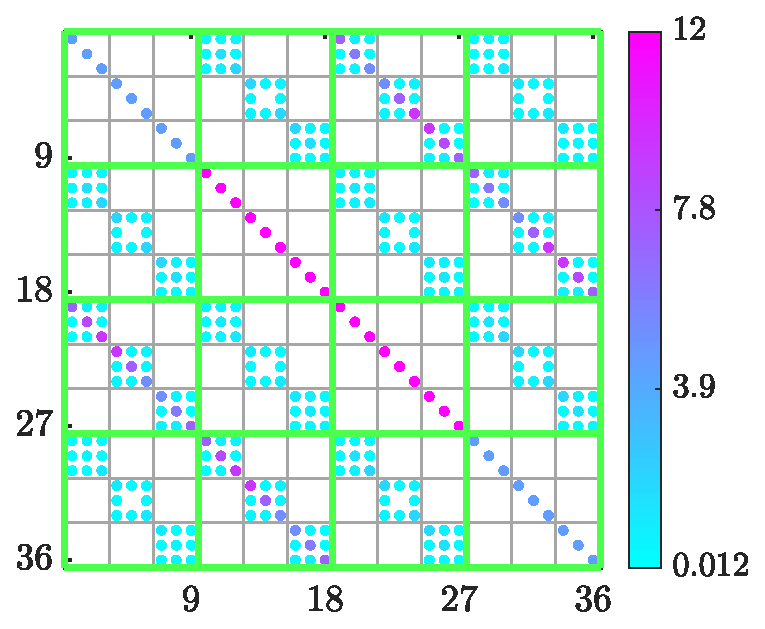
\includegraphics[width=\textwidth]{plots/absG_glob_w_GL_w_CAP.eps}
        \caption[]%
        {{\small $W_0<0$, Methode G2.}}
        \label{fig:G_1}
    \end{subfigure}
    \hfill
    \begin{subfigure}[b]{0.462\textwidth}
        \centering
        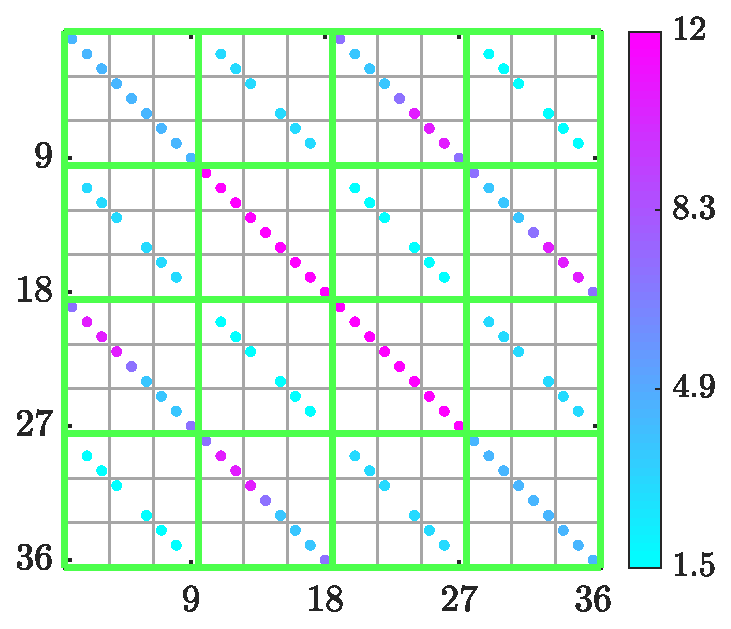
\includegraphics[width=\textwidth]{plots/absG_glob_wo_GL_w_CAP.eps}
        \caption[]%
        {{\small $W_0<0$, Methode G1.}}
        \label{fig:G_2}
    \end{subfigure}
    \vskip\baselineskip
    \begin{subfigure}[b]{0.488\textwidth}
        \centering
        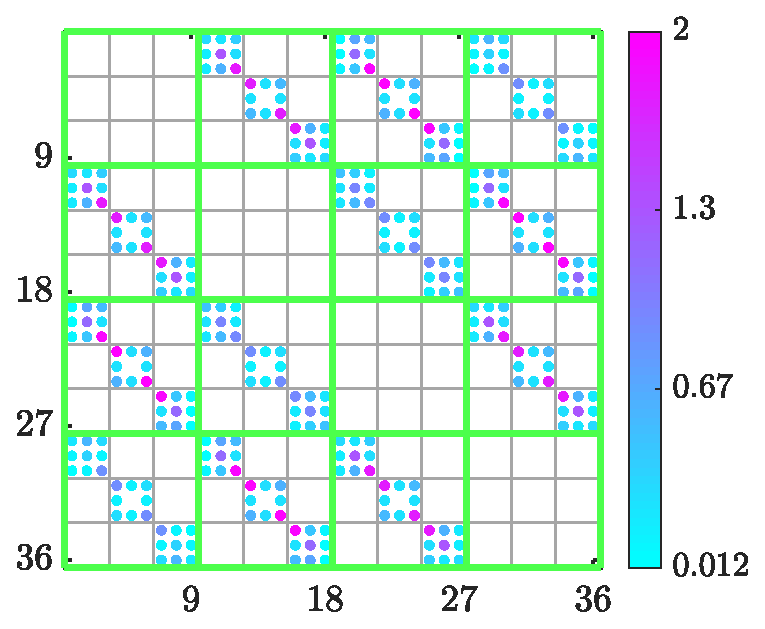
\includegraphics[width=\textwidth]{plots/absG_glob_w_GL_wo_CAP.eps}
        \caption[]%
        {{\small $W_0=0$, Methode G2.}}
        \label{fig:G_3}
    \end{subfigure}
    \quad
    \begin{subfigure}[b]{0.462\textwidth}
        \centering
        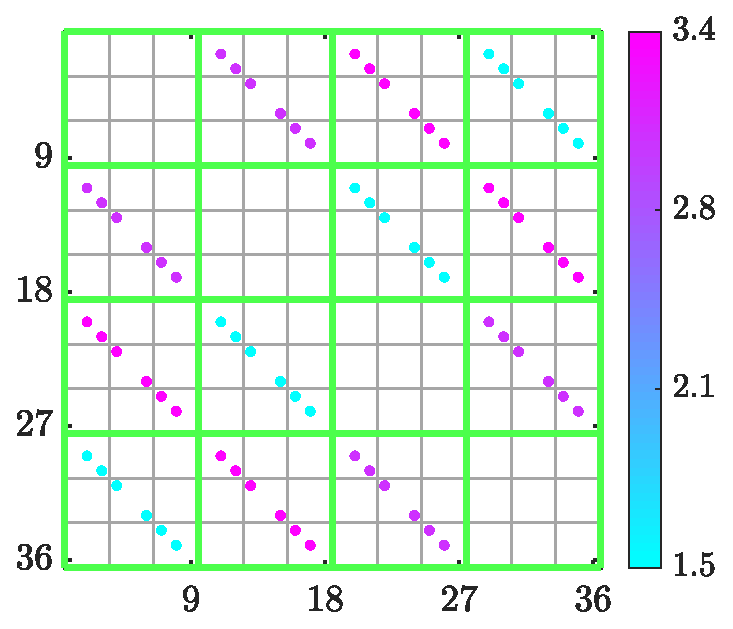
\includegraphics[width=\textwidth]{plots/absG_glob_wo_GL_wo_CAP.eps}
        \caption[]%
        {{\small $W_0=0$, Methode G1.}}
        \label{fig:G_4}
    \end{subfigure}
    \caption[]
    {Betrag der Driftmatrix für verschiedene Fälle in willkürlichen Einheiten. Die beiden linken Teile sind mit Gauß-Lobatto Quadratur berechnet, rechtsseitig ist das Produkt $G(x)v\fin(x)$ in der nodalen Basis entwickelt worden (siehe oben). Für die beiden oberen Teile ist das \ac{cap} eingeschaltet (vgl. \eqref{eq:CAP}), unten ist es ausgeschaltet.}
    \label{fig:matrix_G}
\end{figure*}
Zunächst ist hierzu anzumerken, dass die Matrix den einzig komplexen Beitrag zur Systemmatrix liefert -- gezeigt ist an dieser Stelle lediglich der Betrag. Das \ac{cap} liefert wesentliche Beiträge, was jedoch in diesem Beispiel der sehr groben Diskretisierung in $y$-Richtung geschuldet ist. Ferner ist die Hauptdiagonale für eine feinere Diskretisierung nicht unbesetzt wie die Grafik hingegen vermuten lässt. Bemerkenswert ist die nominelle Ähnlichkeit in Bezug auf die Hauptdiagonalen eines jeden grünen Quadrates zwischen Methode G1 und G2. Für Methode G2 kommen erwartungsgemäß Nebendiagonalbeiträge hinzu, siehe Gleichung \eqref{eq:G_GL}. Für die Darstellung ist ein Flachbandpotential gemäß Abbildung \ref{fig:pot1} angesetzt worden, weshalb es zu weiteren erkennbaren Symmetrien in der Struktur kommt.

\subsubsection{Zeitentwicklung} \label{sec:timestepping}  \index{Zeitentwicklung}
Im transienten Fall ist $\partial_t\neq 0$ und daher Gleichung \eqref{eq:stat_LGS} durch
\begin{equation}
  \td{}{t} \underline{v} = -\underline{\underline{\mathcal{A}}}\, + \underline{b} \equiv\mathcal{F}(\underline{v},t)
  \label{eq:system_transient}
\end{equation}
zu ersetzen. Dieser letzte Schritt überführt die semidiskrete Form aus Abbildung \ref{fig:methodeDerGeraden} (Punkt C) in die vollständig diskretisierte Form (Punkt D). In der Herleitung des stationären Schemas aus dem vorherigen Abschnitt ist die Gleichung lokal bereits mit $(M^k)^{-1}$ multipliziert worden. Da die Massenmatrix bezüglich der \ac{dg}-Diskretisierung blockdiagonal ist, ist die Invertierung besonders einfach, weshalb bei \ac{dg}-Verfahren in aller Regel explizite Zeitschrittverfahren zur Anwendung kommen. Dies stellt einen Vorteil gegenüber einem \ac{cg}-Verfahren dar, wo die globale Massenmatrix nicht blockdiagonal ist, vergleiche auch Kapitel \ref{sec:Übersicht}. Gegenüber impliziten Verfahren sind die expliziten Verfahren in der Regel schneller \cite{LeVeque}.

Deshalb sind in der vorliegenden Arbeit zur Lösung des Systems gewöhnlicher Differentialgleichungen \eqref{eq:system_transient} \ac{rk}-Verfahren der Ordnung zwei und vier (\ac{rk}2 und \ac{rk}4) implementiert worden. Zu Testzwecken ist dabei das Verfahren zweiter Ordnung als \emph{strong stability preserving} ausgelegt, das heißt es erhält die sogenannte TVDM-Eigenschaft:
\begin{equation*}
  \sum_{D^k\in\mathcal{T}\textbackslash D^{K_x}} |\bar{v}\fin^{k+1,n+1} - \bar{v}\fin^{k,n+1}| \leq\sum_{D^k\in\mathcal{T}\textbackslash D^{K_x}} |\bar{v}\fin^{k+1,n} - \bar{v}\fin^{k,n}| \; .
\end{equation*}
Hierbei ist $\bar{v}\fin^{k,n}$ der Mittelwert von $v\fin$ in Zelle $k$ im Zeitschritt $n$. Dazu werden \emph{Limiter} hinzugeschaltet, die nach jedem Zeitschritt die Steigung der Lösung innerhalb der Zellen leicht korrigiert, um diese Eigenschaft zu garantieren. Mit solchen Verfahren sollen unphysikalische Überschwinger vor Allem bei nichtlinearen \ac{pdgn} mit unstetigen Lösungen verhindert werden. Näheres ist in der Literatur \cite{buch} zu finden.

Das \ac{rk}2-Verfahren genügt der Vorschrift
\begin{equation}
  \begin{aligned}
    p^{(1)} &= v\fin^n + \Delta t \mathcal{F}(v\fin^n,t^n) \\
    v\fin^{n+1} = \frac{1}{2}(v\fin^n + p^{(1)} + \Delta t \mathcal{F}(p^{(1)},t^n+\Delta t)) \; ,
  \end{aligned}
\end{equation}
wobei die Länge eines Zeitschrittes in Abhängigkeit von Polynomgrad $N$ der \ac{DG}-Diskretisierung sowie den Gitterabständen $h_x$ (als Mittelwert der $h^k$) und $h_y$ gewählt werden sollte. Hierzu gibt es keine analytische Vorschrift, sondern es gilt die Daumenregel \cite{buch}
\begin{equation}
  \Delta t \leq \frac{1}{2N+1}c\frac{h_x}{h_y \text{max}(\Lambda)}
\end{equation}
mit einer Konstanten $c$, die durch numerische Experimente für das \ac{rk}2-Verfahren zu $c=0.2$ und für das \ac{rk}4-Verfahren entsprechend verdoppelt zu $c=0.4$ gewählt wird. Das \ac{rk}4-Verfahren wird in der geläufigen speicherarmen Version
\begin{equation}
  \begin{aligned}
    p^{(0)} = v\fin^n \\
    i\in [1,\dots,5]: \begin{cases}
      q^{(i)} = a_i q^{(i-1)} + \Delta t \mathcal{F}(p^{(i-1)},t^n+c_i \Delta t) \\
      p^{(i)} = p^{(i-1)}+b_iq^{(i)}
  \end{cases} \\
  v\fin^{n+1} = p^{(5)}
  \end{aligned}
\end{equation}
implementiert. Die Koeffizienten $a_i,b_i,c_i$ können der Literatur \cite{buch} entnommen werden. Offenbar werden in dieser Variante fünf Funktionsaufrufe benötigt, was zunächst gegenüber der Ordnung des Verfahrens einen Mehraufwand bedeutet. Dadurch jedoch können größere Zeitschritte $\Delta t$ realisiert werden \cite{buch}.
% Die in Abbildung \ref{fig:pot1} eingezeichneten Längen werden wie in \cite{lukas1} zu
% \begin{align}
%   L_1 &= \SI{6}{\nano\meter}\\
%   L_2 &= \SI{5}{\nano\meter}\\
%   L_U &= \SI{30}{\nano\meter} \; .
% \end{align}
% gewählt. Hierin ist $L_U$ die Länge, über der die Spannung $U$ abfällt.

% \todo{Idee: TF-Lösung für Überlagerung von l und r zeigen.}

% \section{Mathematische Aspekte der \lvn}
% Die eindimensionale Wellenfunktion $\Psi(x)$ eines Teilchens ist ein Vektor des unendlich-dimensionalen Hilbertraums $L^2(\mathbb{R})$ mit dem üblichen Skalarprodukt
% \begin{align}
%   \bra{\Psi}\ket{\Phi} = \int_{\mathbb{R}} \Psi^*(x)\Phi(x) \diff x \; .
% \end{align}
% Beschränken wir uns auf ein Rechengebiet $L$, so ist entsprechend $\Psi(x) \,\in\,L^2(L)$. Diskretisieren wir ferner das System, so wird der Hilbertraum endlichdimensional mit Dimension $N$. Dann ist die Dichtematrix in Gleichung \eqref{eq:lvn} eine Matrix der Form $\mathbb{C}^N \times \mathbb{C}^N$ und der Liouville-Operator ein "Superoperator" \cite{frensley2} der Form $(\mathbb{C}^N \times \mathbb{C}^N)\times(\mathbb{C}^N \times \mathbb{C}^N)$.
% Letztlich wird numerisch gesehen $N^2$ der Anzahl Freiheitsgrade entsprechen und die \lvn wird wieder eine Matrix-Vektor-Gleichung sein. Dazu wird $u(x,y)$ nicht als Matrix, sondern als Vektor der Länge $N^2$ geschrieben.
% \todo{Eigenschaften von B(x,y) und A. Hermitizität von $\mathcal{L}$ (frensley).}
